\chapter[Filesystem]{Filesystem \\ \Large \textnormal{François Costa}}

\section{Overview of the architecture}

\begin{itemize}
    \item \textbf{fopen.c}: This file represents the high-level library and is the inteface with other processes, facilitating their interaction.

    \item \textbf{aos\_rpc.c}: Serves as a bridge between the high-level library and the FAT32 filesystem, this file handles the communication between shared libraries and FAT32. It ensures the maintenance of invariants enforced by the disk.

    \item \textbf{fat32.c}: Is responsible for the implementation of the FAT32 filesystem, this file provides the necessary services to maintain the required invariants.

    \item \textbf{blockdriver.c}: Is acting as the block driver, this file handles the actual communication with the disk, serving as a vital component of the overall system.

    \item \textbf{fat32\_test.h}: During the compile time, this header-only file, which serves the purpose of testing the filesystem, is incorporated into \texttt{fat32.c}. This file isn't present in the production code.

\end{itemize}

The initial section provides an overview of the high-level architecture used for the implementation. In the filesystem implementation, several files assume significant roles:
 
\begin{figure}[htp]
    \centering
    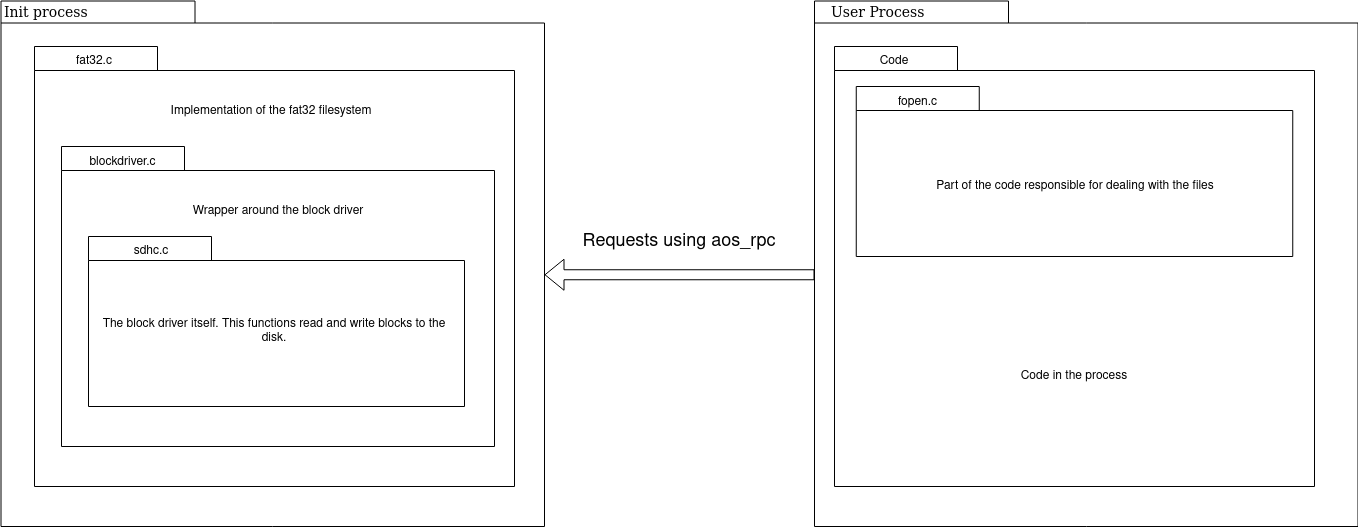
\includegraphics[width=12cm]{images/filesystem/high_level overview.drawio.png}
    \caption{High level overfiew of the architecture}
    \label{fig:galaxy}
\end{figure}


\subsection{Each module has its own scope}
In the system architecture, each C file holds specific responsibilities. We can make a clear distinction between them. The block driver communicates with the disk, ensuring smooth data transfer. The FAT32 filesystem focuses on maintaining the necessary invariants required by the filesystem itself. Lastly, the RPC framework takes charge of communication between the system and external entities, providing a way to interact with the rest of the world.

\subsection{The block driver and the filesystem are bound together}

An architectural decision that is very important is the \textbf{coexistence} of the block driver and the FAT32 filesystem within the same process (init), eliminating the need for RPC (Remote Procedure Call) communication between them. The filesystem holds a pointer to the driver block, enabling direct communication with the disk. While the filesystem assumes the responsibility of \textbf{maintaining the disk's invariants}, the block driver handles the actual \textbf{disk communication}. Both components operate within the init process as part of a larger system-wide design paradigm. By consolidating all services within init and directing all RPC requests to it, this design choice aligns with the overall system architecture (see LMP section for more details). Consequently, the filesystem architecture follows the notion of not reinventing the wheel, utilizing existing components efficiently.

This architectural decision was carefully made to ensure \textbf{consistency} across the entire system. Maintaining consistency is important as it promotes coherence, predictability, and compatibility among different components and processes within the system.

\subsection{The filesystem maintains the required invariants in a fat32 filesystem}

At the core of this architecture lies a core concept: establishing a \textbf{singular point of trust} for maintaining the essential invariants required by the FAT32. This responsibility rests solely with the internal workings of the FAT32 itself, which effectively utilizes the block driver to establish communication with the disk. As a consequence, any request pertaining to the filesystem must follow a prescribed path, traversing through the init process and, more specifically, the FAT32 filesystem component (\texttt{fat32.c}). This design ensures a \textbf{centralized} and controlled approach to filesystem operations, reinforcing reliability and security.

The FAT32 assumes the crucial role of being the sole entity we rely on to uphold the necessary invariants within the disk. It becomes the singular point of trust, responsible for maintaining the integrity and consistency of the filesystem. By placing our trust in the FAT32, we ensure that all required invariants are preserved, providing confidence in the reliability and stability of the disk.

\subsection{Finally, a solid test infrastructure}

The file fat32\_test.h plays a crucial role in our system as it serves as the central place for executing all unit tests. Its responsibility lies in ensuring the \textbf{integrity} and functionality of various components within the system. Whenever a new feature is added or a function is modified, leveraging the tests becomes a valuable practice. These tests act as a safety net, allowing us to validate that the changes made do not introduce unforeseen issues or regressions into the system. Running the tests following a modification or addition helps ensure that the system continues to operate smoothly and as intended.

After successfully validating a set of tests, I extracted a subset from them and designed a new process to replicate the same operations. While the decision to reuse the same tests may appear unconventional, there exists a logical rationale behind it. Employing different tests could potentially unveil additional scenarios to verify, but in the event of an error, it becomes challenging to discern whether it originates from inter-process communication or the FAT32 itself. By utilizing identical tests, we expedite the bug detection process, as the high probability lies within the RPC layer. This approach significantly accelerates bug discovery, enabling prompt resolution and debugging of the system.

\begin{lstlisting}[caption={Unit tests executed},captionpos=b,language=C,frame=single,breaklines]
void _test_name_len(void);
void _test_extension_len(void);
void _test_name_valid(void);
void _test_compare_entries_call(const char *name_entry, const char *extension_entry, const char *name, bool expect);
void _test_compare_entries(void);
void _test_shortname_to_name(void);
void _test_name_to_shortname(void);
void _test_resolve_call(struct fat32_filesystem *fs, const char *test_name, const char *path, bool result);
void _test_resolve(struct fat32_filesystem *fs);
void _test_fopen(struct fat32_filesystem *fs, const char *path);
void _test_freadseek(struct fat32_filesystem *fs, const char *path);
void _test_fwrite(struct fat32_filesystem *fs, const char *path);
void _test_fwrite_huge(struct fat32_filesystem *fs, const char *path);
void _test_mk_rm(struct fat32_filesystem *fs, const char *dir);
void _test_create_write_remove(struct fat32_filesystem *fs, const char *path);

\end{lstlisting}

\section{The block driver}

\subsection{Technical background}

A block driver is a software component that enables a computer's operating system or processes to communicate with block devices, such as hard drives, solid-state drives, USB flash drives and SD cards.

A block device is a storage device that reads and writes data in fixed-size chunks or blocks. The block driver acts as an interface between the operating system and the block device, allowing the operating system to read and write data to the device. In our case, thanks to the block driver we can see our block device as a gigantic array with each entry as an array of 512 bytes.

The block driver provides a set of functions that allow the operating system to access the block device, including functions to read and write blocks of data, query device properties, and perform other operations. In addition to providing basic access to the block device, block drivers also provide functionality such as caching, buffering, and error handling. Caching and buffering can help improve performance by reducing the number of disk accesses needed to read or write data, while error handling can help ensure data integrity by detecting and correcting errors that occur during data transfer. Caching was implemented as extra challenge.

The driver block we are given is not as powerful and does not have all the features, but it allows to read and write blocks, and this is enough to build a filesystem on top of it. However, caching was implemented as extra challenge.

\subsection{Implementation of the bloc driver}

I have written a file named \texttt{blockdriver.c} that serves as an easy wrapper around the block driver. Within this file, three distinct functions were create to enhance its functionality. Firstly,  a straightforward function that initializes the blockdriver, ensuring its proper setup. Secondly, we have a function dedicated to retrieving blocks of data from the disk, which greatly aids in efficient data retrieval. Finally, the last function within this file is specifically designed to facilitate reading data from the disk, thereby streamlining the reading process. It is worth mentioning that despite its concise length, this implementation showcases no remarkable or peculiar features, as it predominantly serves as a wrapper around the provided bloc driver.

\begin{lstlisting}[caption={Wrapper around the block driver},captionpos=b,language=C,frame=single,breaklines]
struct block_driver {
    struct capref sdhc_cap;
    lvaddr_t sdhc_vaddr;

    struct capref rw_frame;
    lvaddr_t write_vaddr;
    lvaddr_t read_vaddr;
    lpaddr_t write_paddr;
    lpaddr_t read_paddr;

    struct sdhc_s *driver_structure;
};

errval_t launch_driver(struct block_driver *b_driver);

errval_t read_block(struct block_driver *b_driver, int lba, void *block);
errval_t write_block(struct block_driver *b_driver, int lba, void *block);

\end{lstlisting}

\subsection{Performance evaluation}

For the performance evaluation section, I have added two additional functions that handle reading and writing data from the provided block driver, while also measuring the time it takes to complete these operations. There is no magic involved in these functions; they simply start a timer when the reading or writing process begins and stop it once the function finishes its task.

To gauge the actual speed of the block driver, I conducted 500 read operations and 500 write operations for \texttt{benchmarking} purposes. The results are represented in two plots, which display the statistical distribution of the duration, measured in \textbf{microseconds}, for both block writes and block reads. We can see that the result is consistent with some outliers.

\begin{figure}[htp]
    \centering
    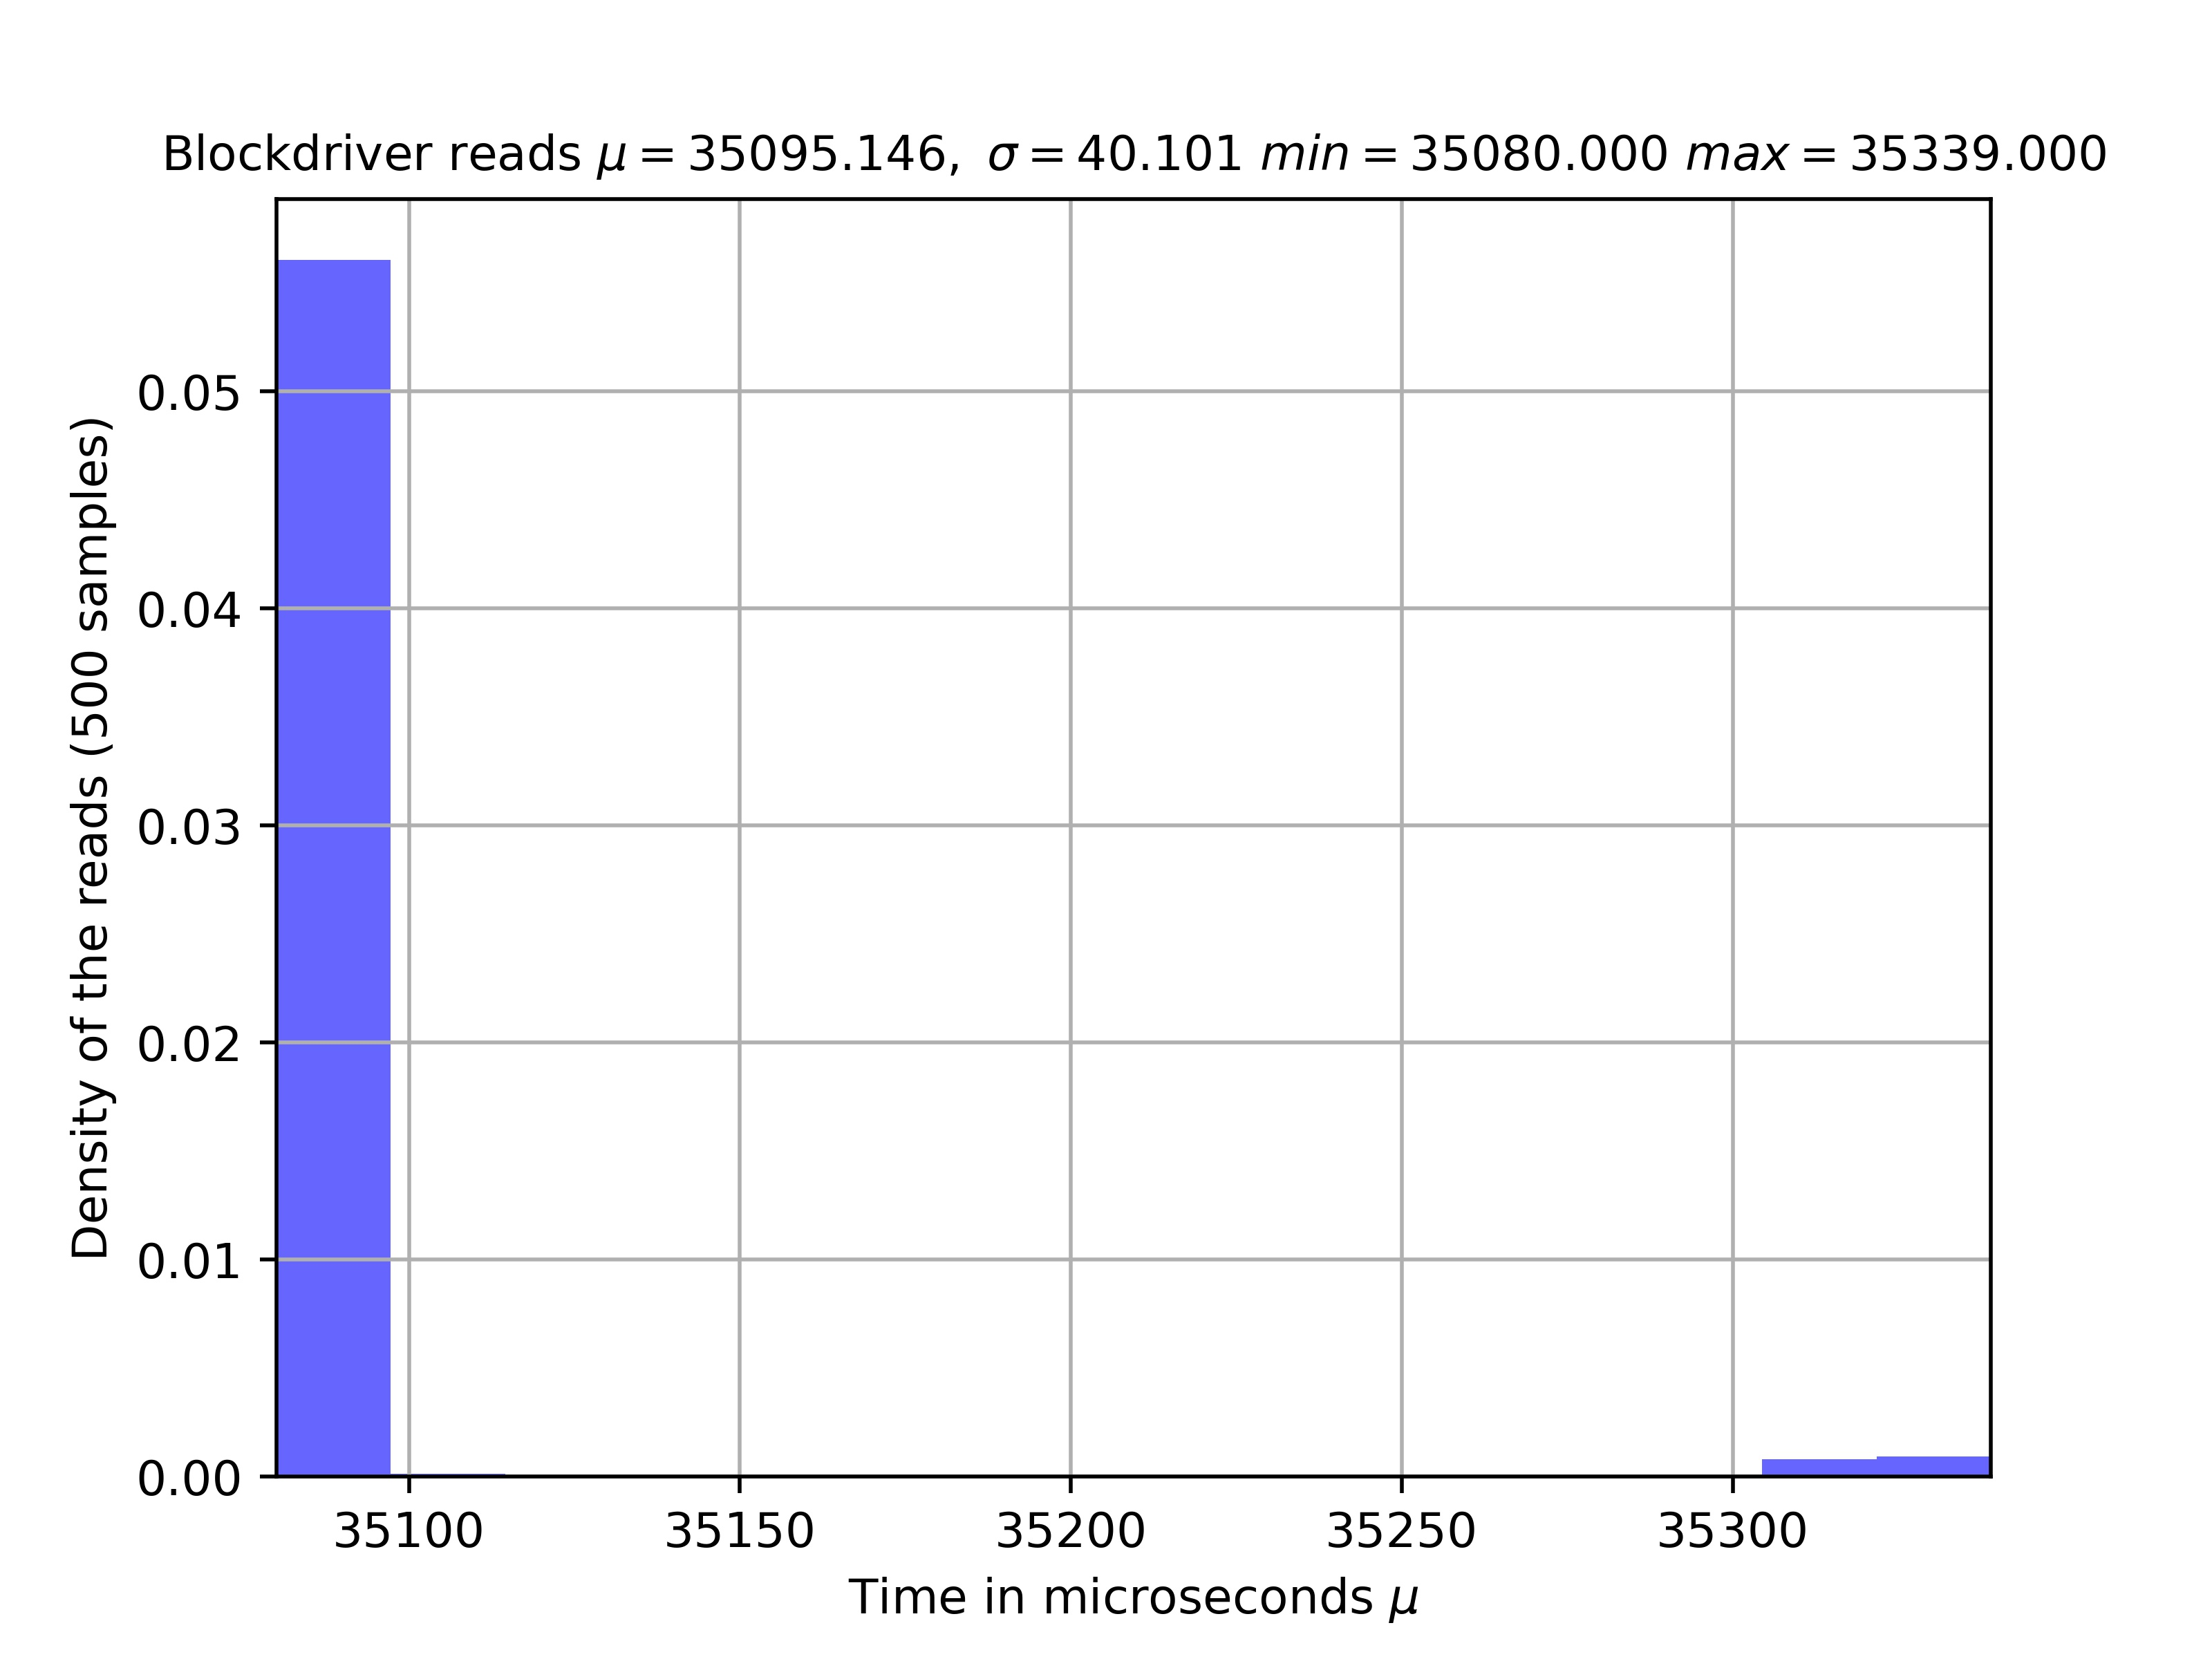
\includegraphics[width=12cm]{images/filesystem/benchmark_read.jpg}
    \caption{Benchmark blockdriver read}
    \label{fig:galaxy}
\end{figure}


\begin{figure}[htp]
    \centering
    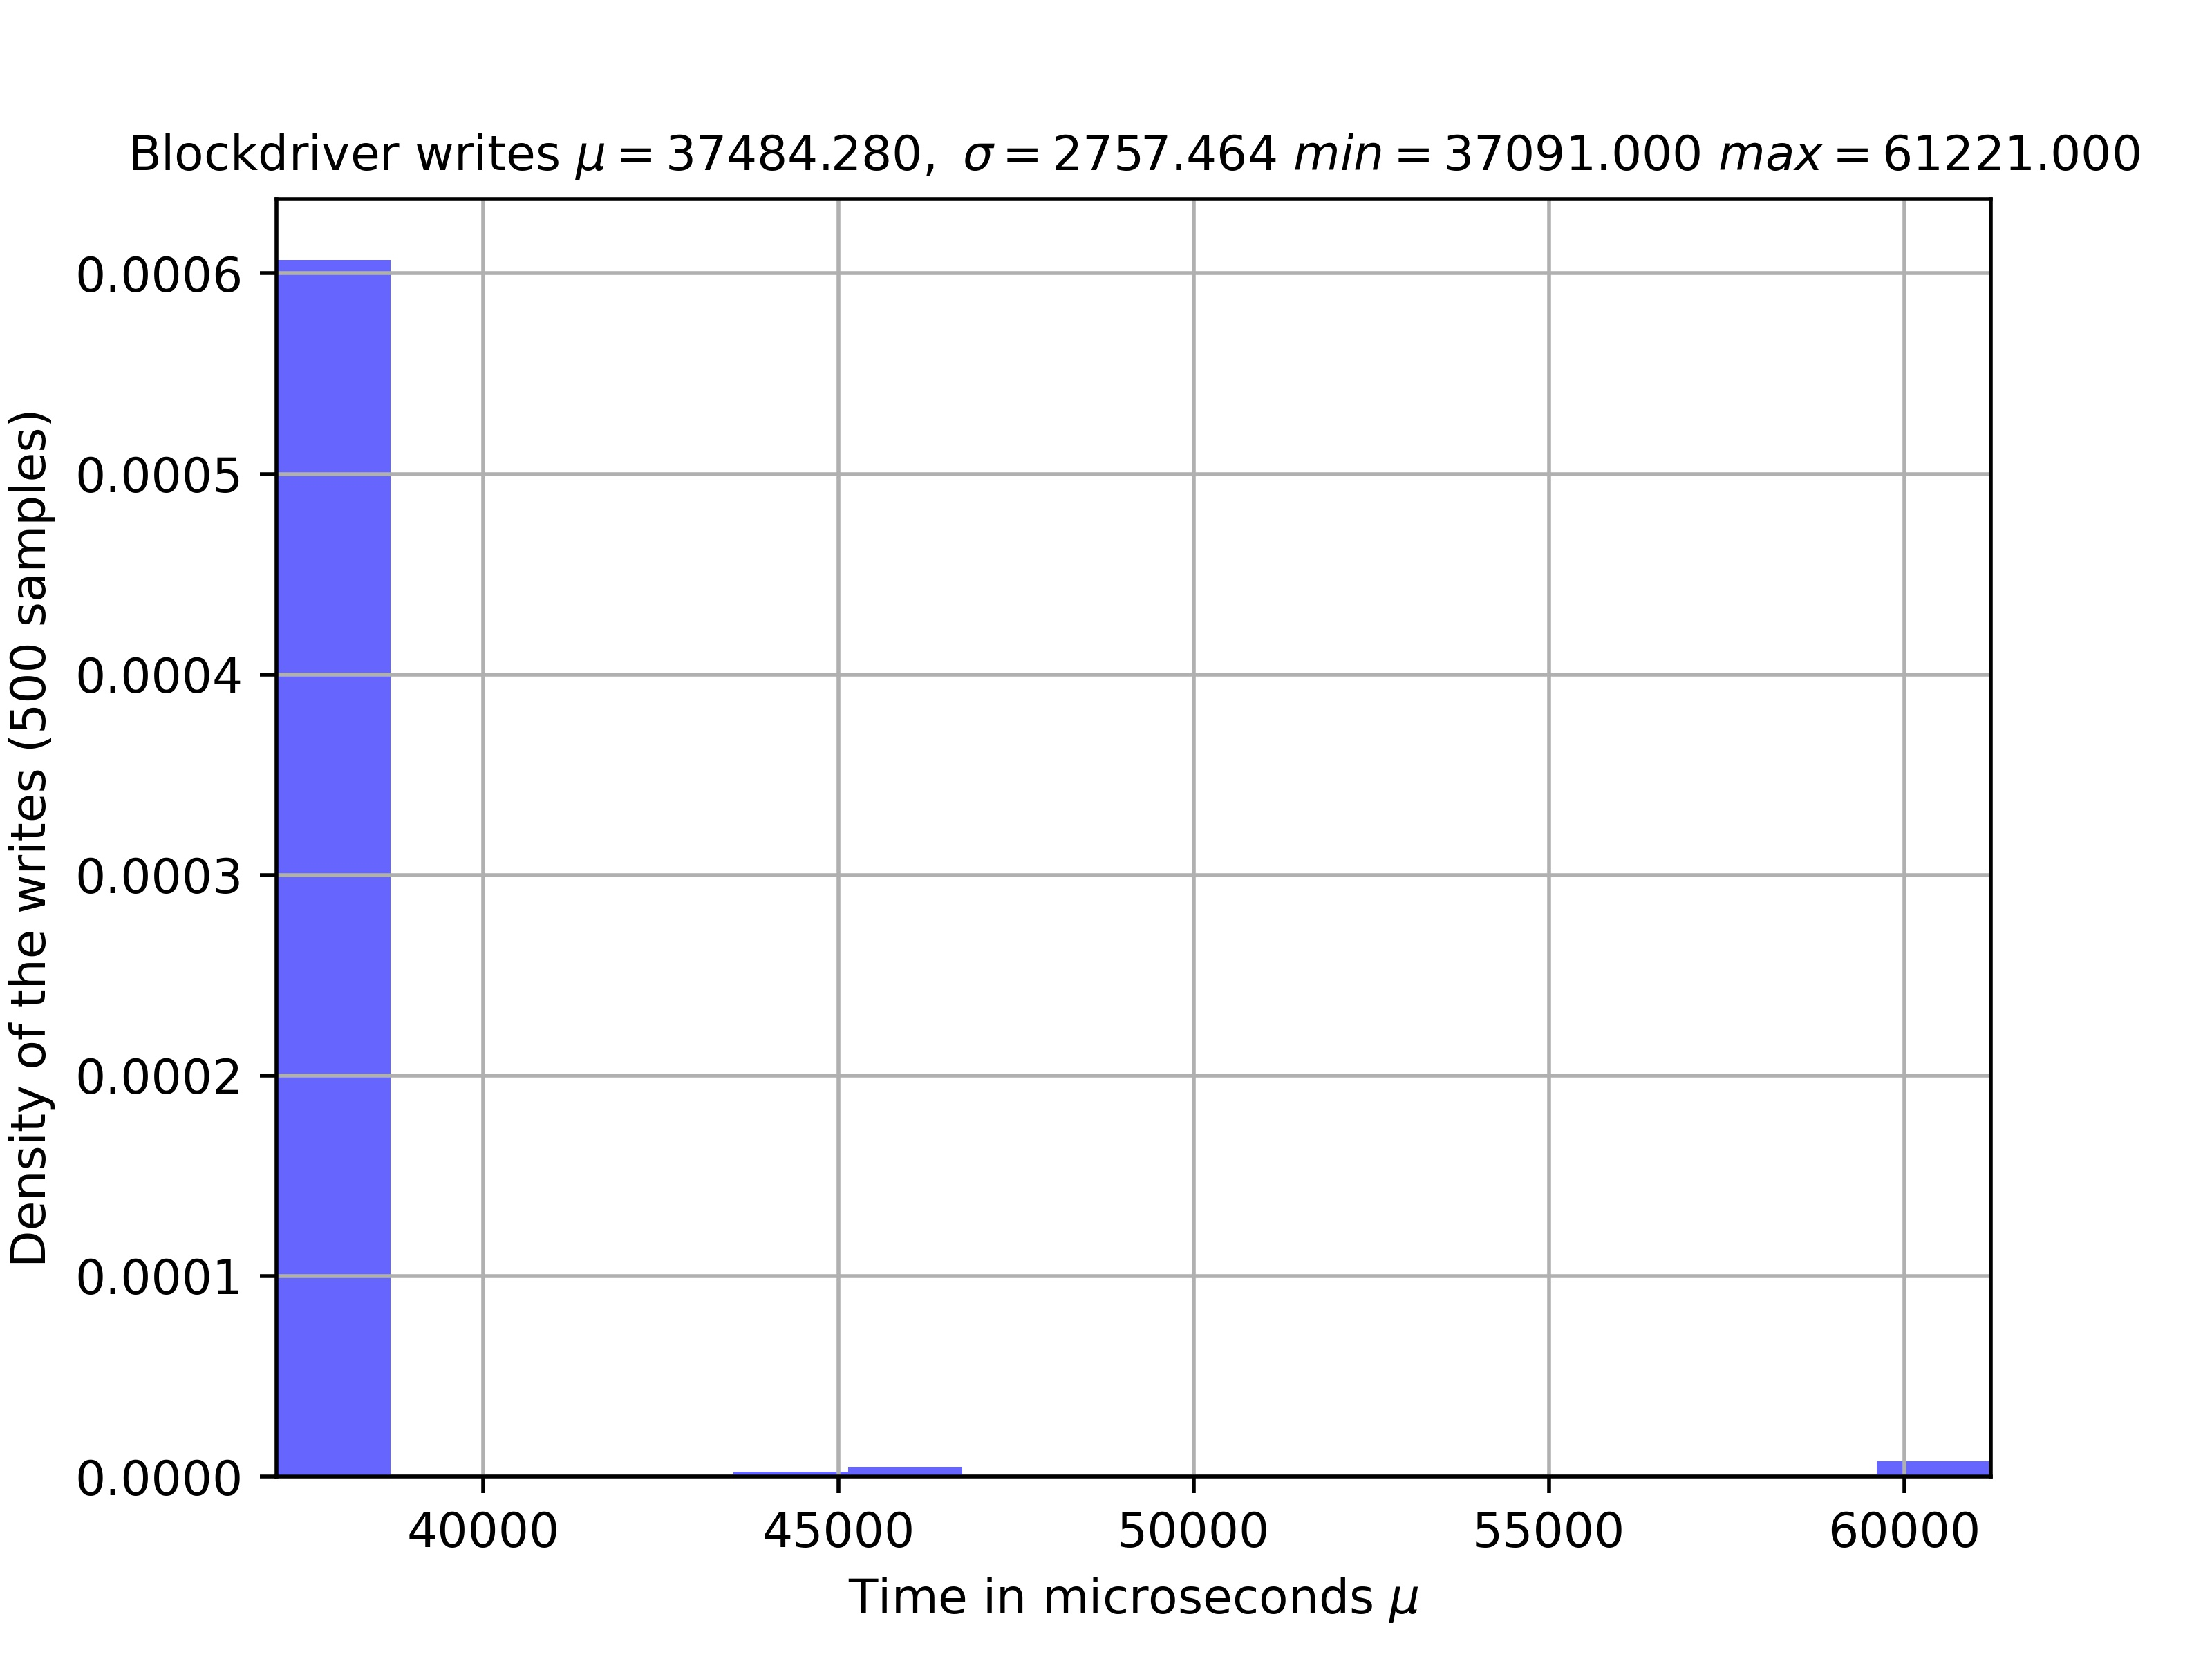
\includegraphics[width=12cm]{images/filesystem/benchmark_writes.jpg}
    \caption{Benchmark blockdriver write}
    \label{fig:galaxy}
\end{figure}

\begin{figure}[htp]
    \centering
    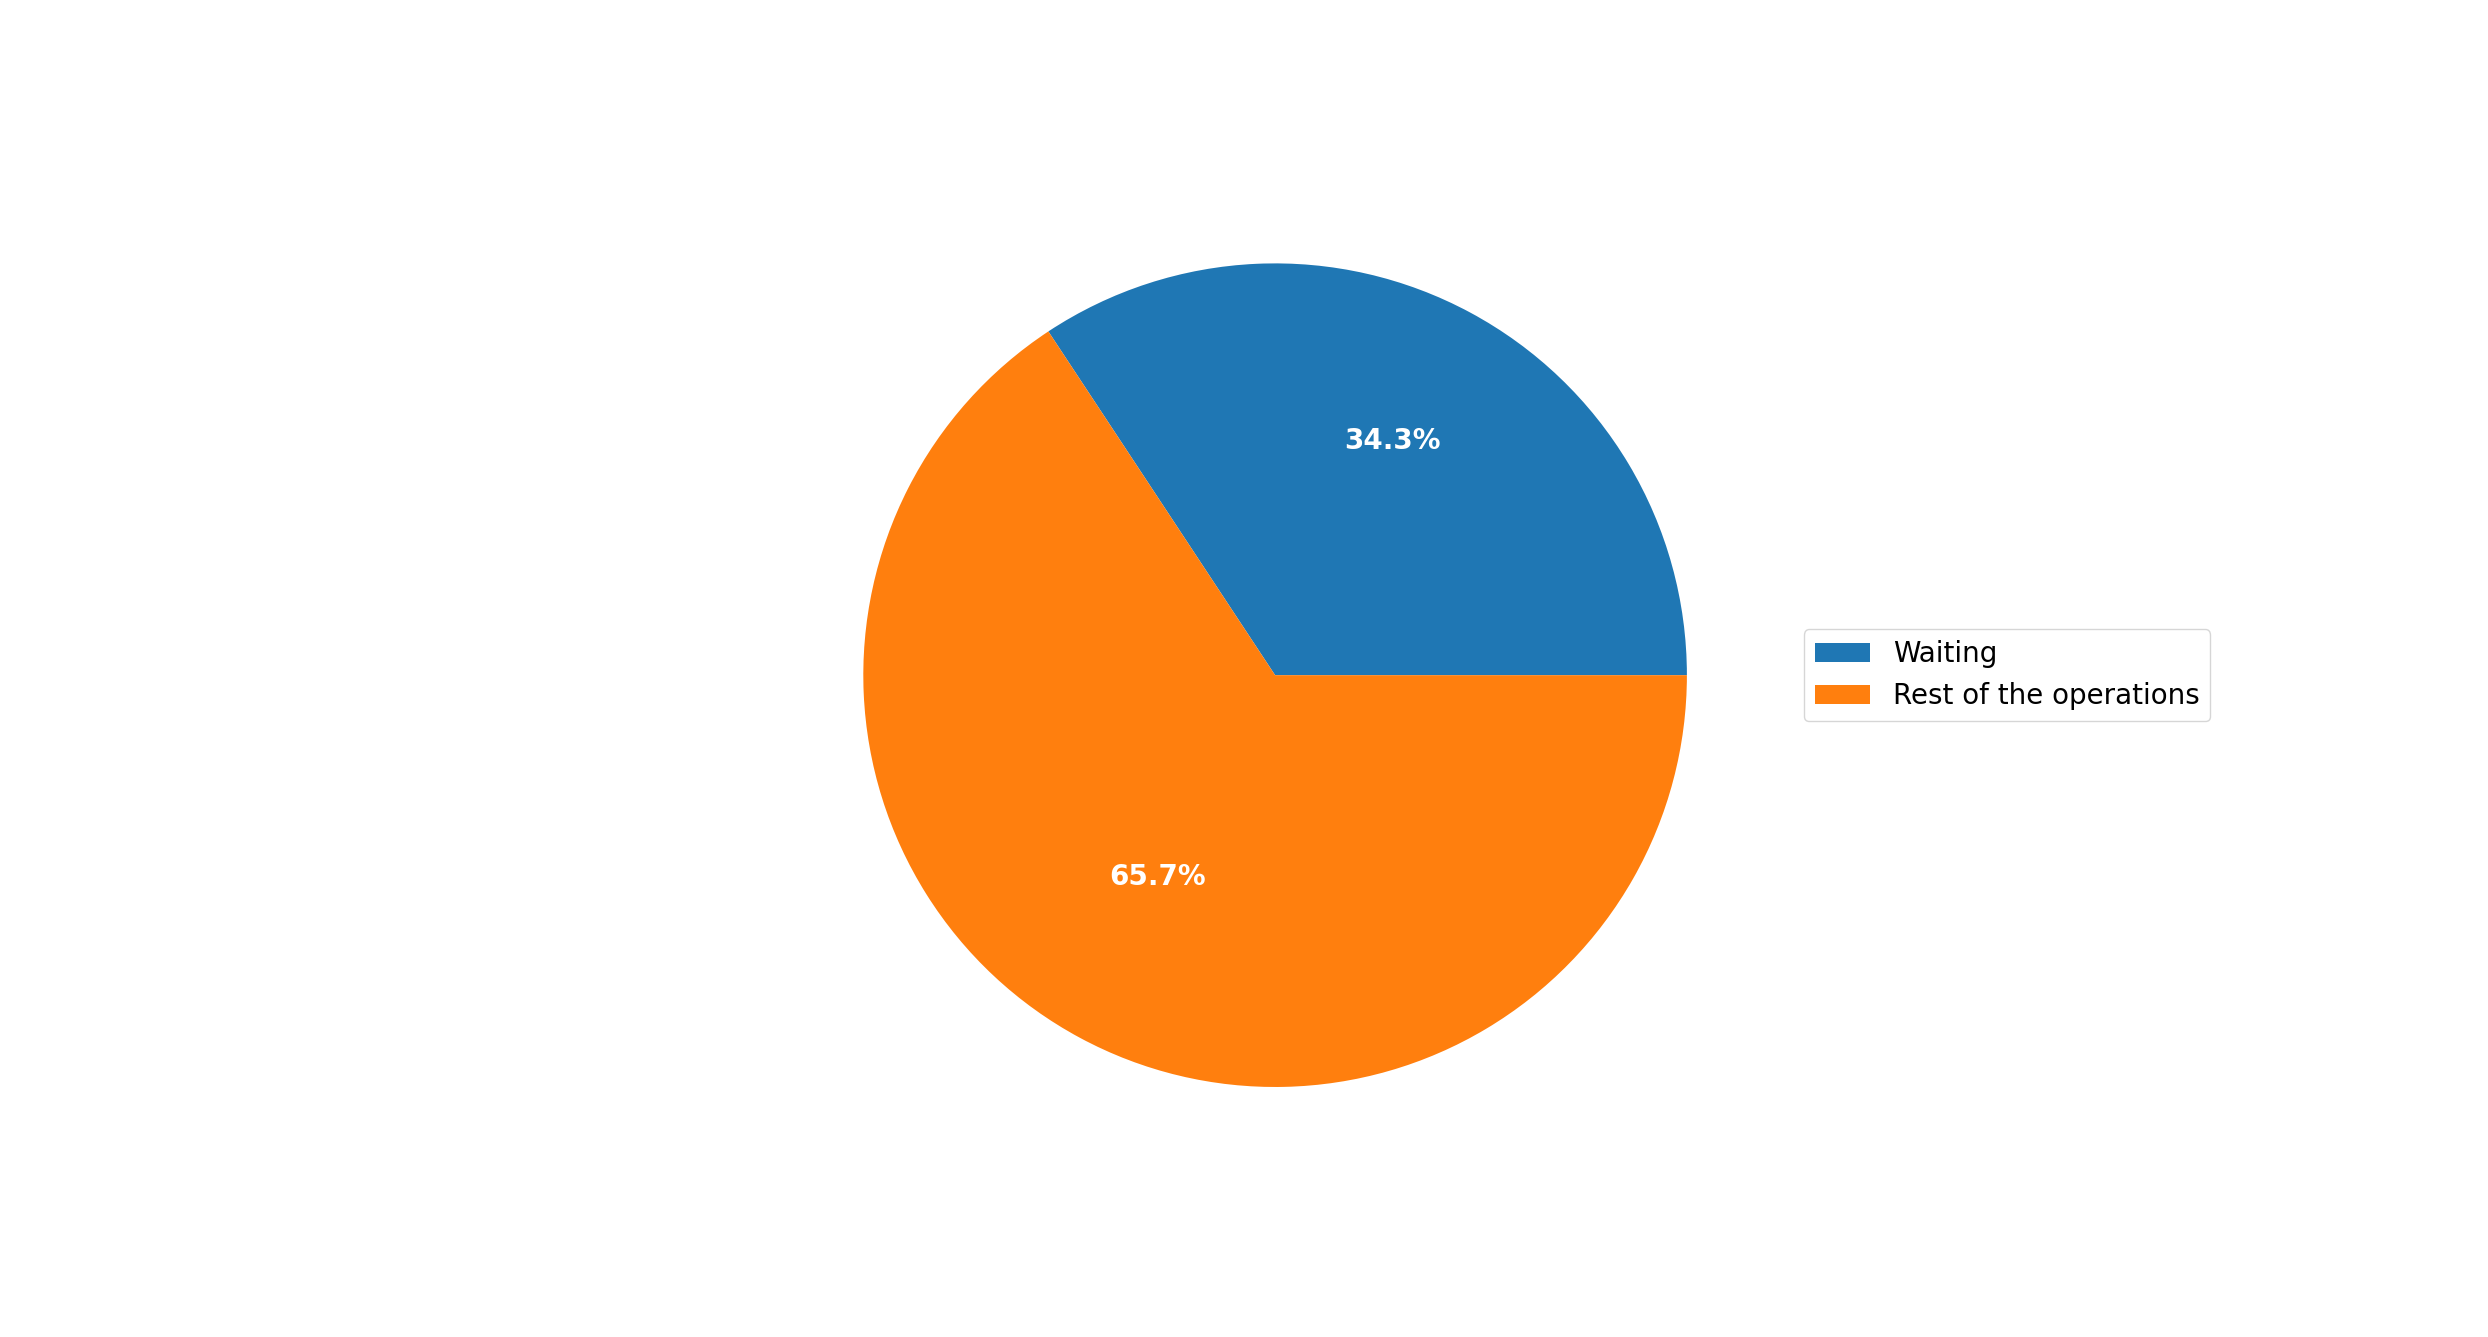
\includegraphics[width=12cm]{images/filesystem/division.png}
    \caption{Time spent in the block driver}
    \label{fig:galaxy}
\end{figure}


\subsection{Extra milestone: Implementing a \href{https://en.wikipedia.org/wiki/Cache_(computing)}{\texttt{software cache}} in the block driver}

When executing the block driver, we observe an interesting yet unsurprising pattern. The \texttt{access pattern} for blocks identified by logical block addressing (LBA) is not random at all. For instance, the \texttt{root cluster} is accessed frequently as it needs to be read each time a path in the filesystem is resolved (further explanations will be provided in the report). In technical terms, this implies the presence of \textbf{temporal locality} in the access patterns, meaning that \textbf{recently accessed elements are likely to be accessed again in the future}.

What does this signify? We are aware that reading from and writing to the disk is exceptionally slow. In the graph displayed below, you can observe the time it takes for these operations. If two blocks are similar, it would be advantageous to find an algorithm or technique to access them only once. As evident from the benchmark results, a computer can accomplish a significant amount of tasks within this time frame. Therefore, it is apparent that we are expending a considerable amount of resources needlessly. To address this issue, we will employ a mechanism known as a \texttt{software cache}.

A \texttt{software cache}. is a mechanism used in computer systems to improve performance by storing frequently accessed data or instructions closer to the processing unit. It acts as a temporary storage area between the CPU and main memory, holding copies of data that are likely to be needed again in the near future. When the CPU requests data, the cache is checked first, and if the data is found, it is retrieved from the cache, which is faster than accessing the main memory. This helps reduce the overall access time and improves system responsiveness by reducing the number of slower memory accesses required.

\begin{lstlisting}[caption={Wrapper around the driver},captionpos=b,language=C,frame=single,breaklines]
void load_driver() {
    // Setup the base driver
    init_driver();
    
   	// Init software cache
    init_cache();  
}

void read_block(size_t lba, void *block) {
    if(try_read_from_cache(lba, block)) {
      return; // Cache hit
    }

    // I/O from disk
    driver_read(lba, block);

    // Update software cache
    update_cache(lba, block);

    return;
}

void write_block(size_t lba, void *block) {
	// Invalidate cache
    invalidate_cache(lba);
  
    // Write-back
    driver_write(lba, block);
  
    return;
}
\end{lstlisting}

Considering the cache size, a cache of size 512 would likely provide better overall performance compared to a cache size of 2048 (current). Increasing the cache size allows for more data to be stored closer to the processor, potentially reducing the frequency of cache misses and improving execution speed. However, further investigation and testing are necessary to determine the optimal cache size for specific workloads.

Regarding the eviction policy, while \href{https://en.wikipedia.org/wiki/Cache_replacement_policies}{\texttt{LRU}} (Least Recently Used) is commonly used and generally effective, it may not always be the best choice for every scenario. Other eviction policies, such as LFU (Least Frequently Used) or Random, may yield better results depending on the specific access patterns and workload characteristics. Determining the ideal eviction policy would require more exploration and experimentation. The cache implements a LRU eviction policy.

Additionally, it's worth noting that the implemented cache follows a \texttt{write-through} policy, meaning that write operations are directly propagated to the main memory. While a \texttt{write-back} cache, which stores modified data in the cache itself before updating the main memory, can provide faster performance for frequent small read and write operations, it introduces additional considerations.

One concern with a write-back policy is the potential delay during operating system shutdown. Flushing the software cache at this point could be time-consuming. Moreover, assuming there is a bug in the operating system or a power failure, data written to the cache but not yet flushed to the main memory would be lost. This behavior is undesirable.

When examining write hits, a significant disparity between read and write speeds becomes evident. This discrepancy is clearly illustrated in the subsequent plot, where a notable increase in speedup is observed. To accurately measure the actual access time, the following formula can be utilized. The parameter $\lambda$ represents the cache \texttt{hit rate}.

\[ f(\text{{access pattern}}) = \lambda \times \text{{hit time}} + (1 - \lambda) \times \text{{miss time}} \]



\begin{figure}[htp]
    \centering
    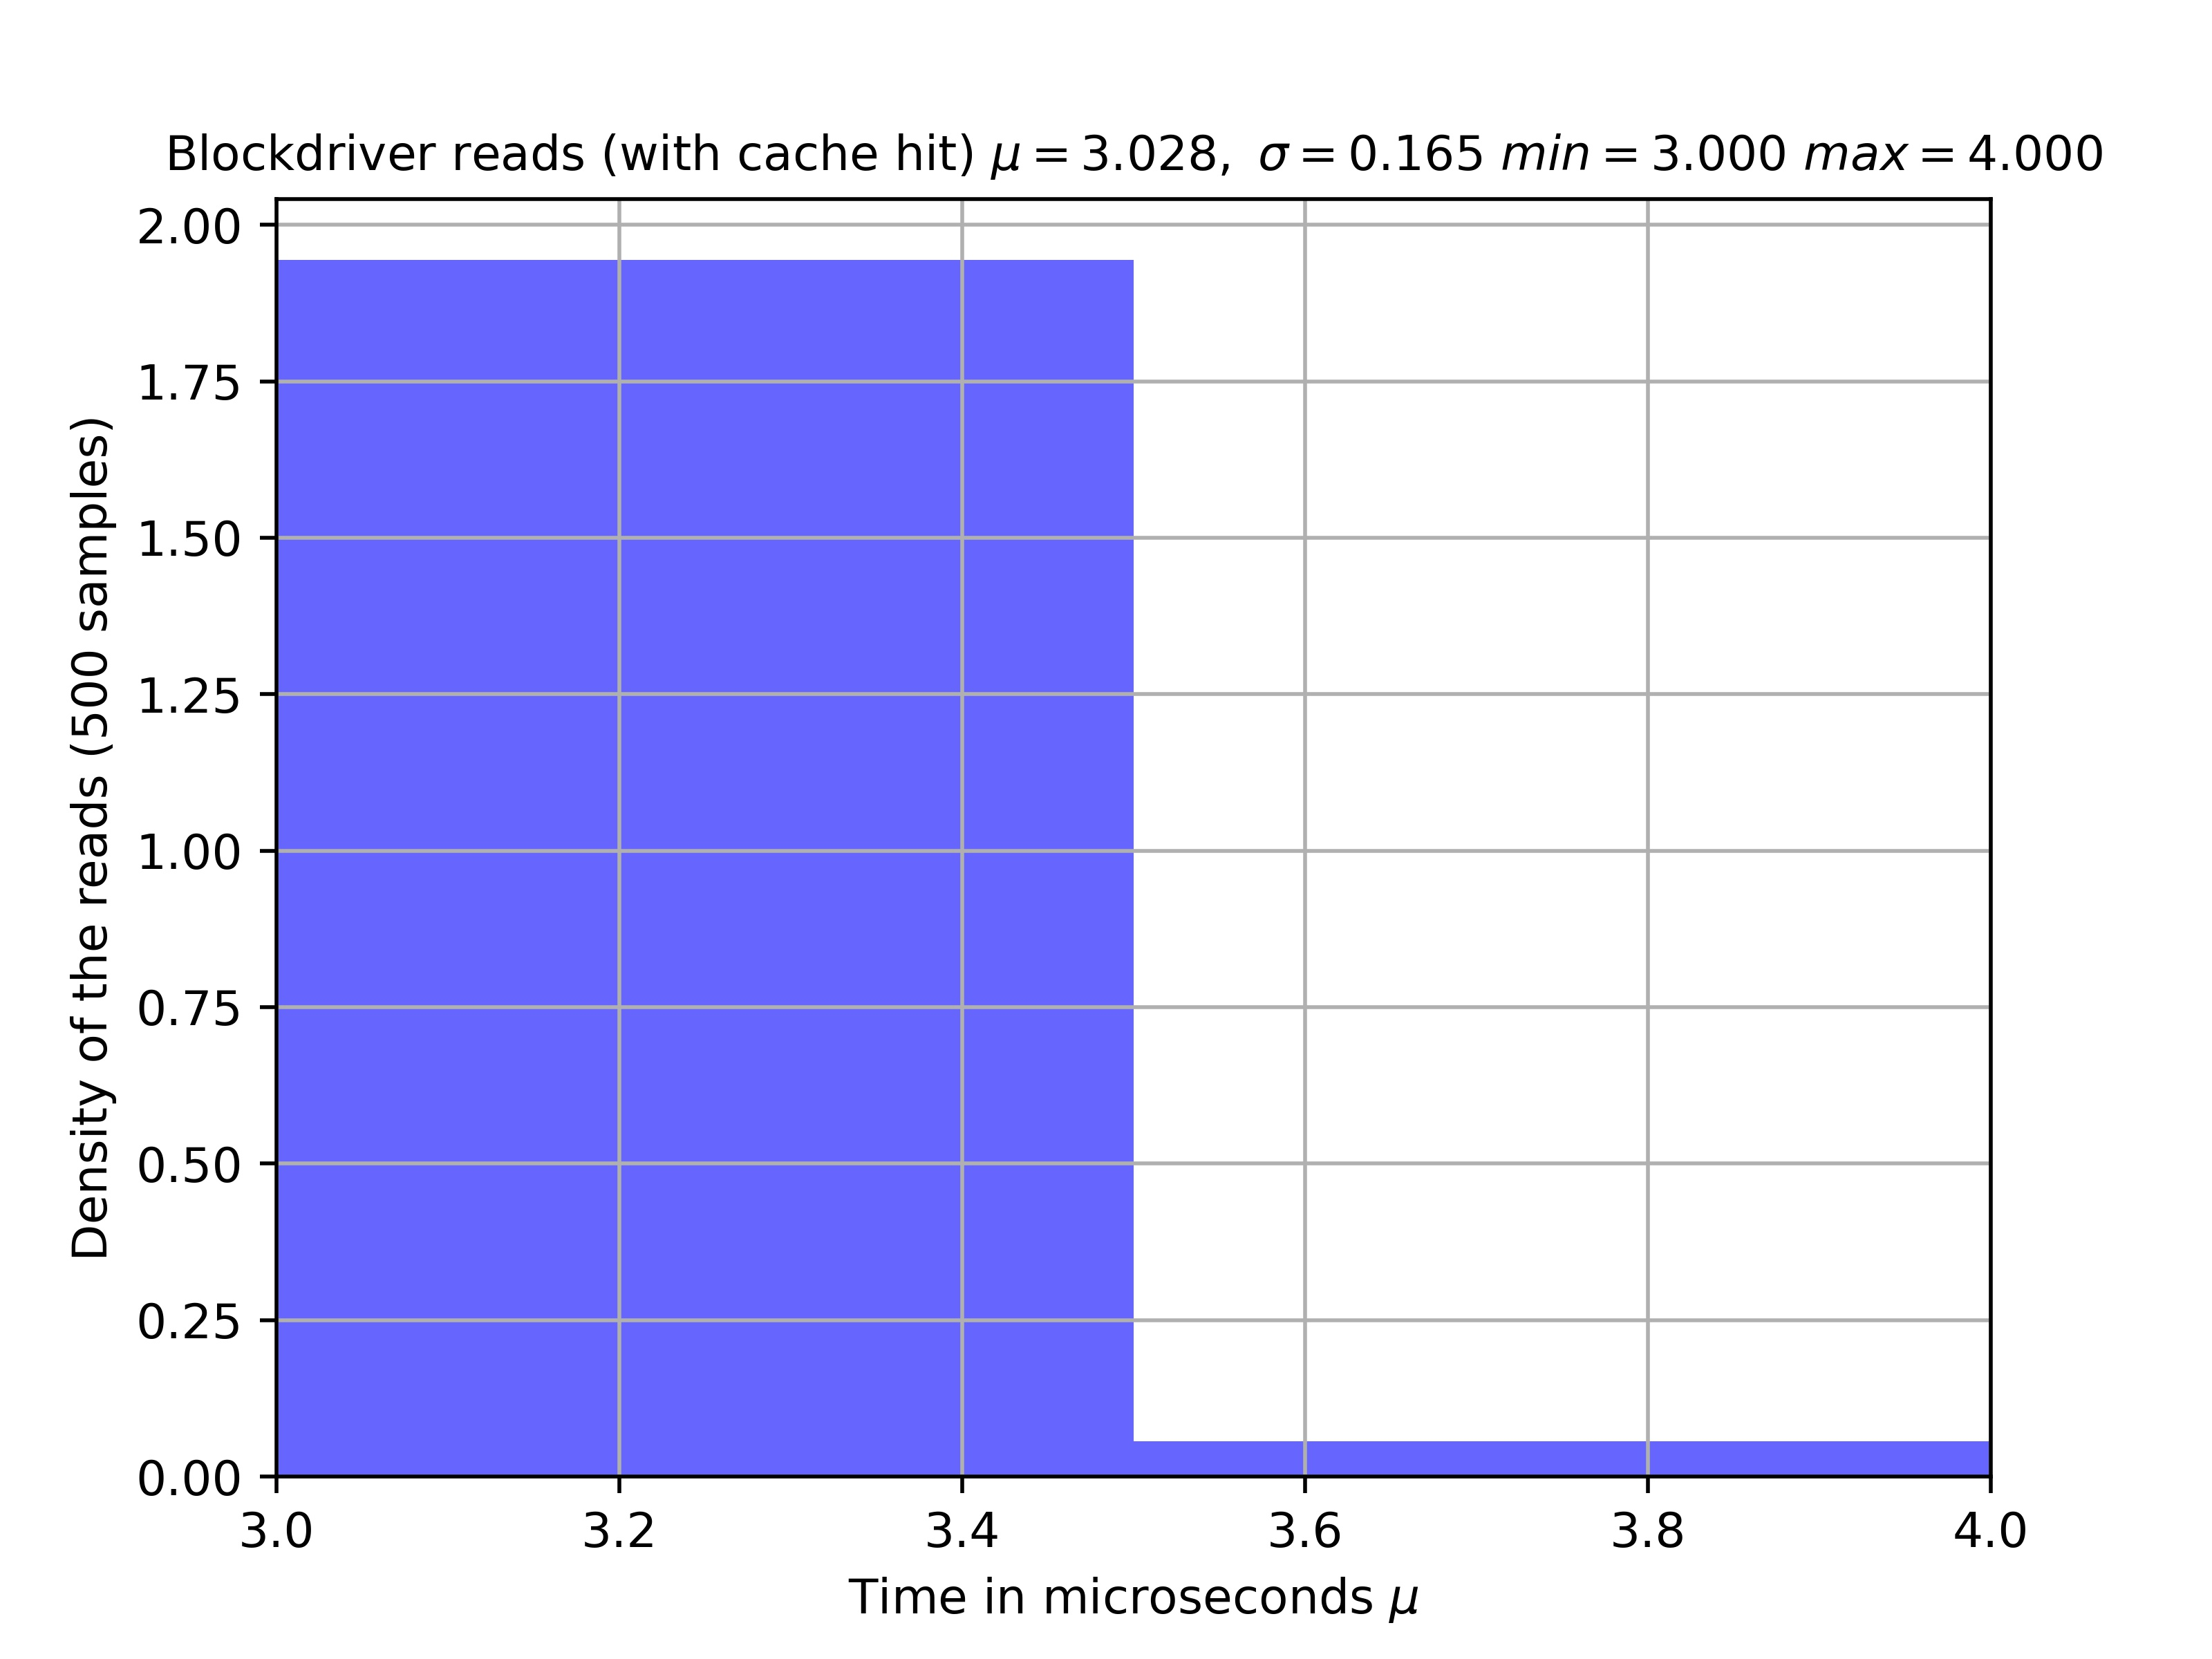
\includegraphics[width=12cm]{images/filesystem/benchmark_read_cache.jpg}
    \caption{Read in the filesystem with cache hit}
    \label{fig:galaxy}
\end{figure}


\section{The Filesystem}

\subsection{What is a filesystem}

In computer science, a \href{https://en.wikipedia.org/wiki/File_system}{\texttt{file system}} is a method of organizing and storing data on a computer's storage devices, such as hard drives, solid-state drives, and USB flash drives. A file system provides a way to organize and access data by creating a \textbf{hierarchical structure} of files and directories.
At its most basic level, a file system provides a way to store and retrieve files on a storage device. However, modern file systems also provide additional functionality, such as file permissions and security features, support for different file types and data compression, and data recovery features.
\begin{itemize}
A file system typically consists of several key components, including:
    \item Data structures: A file system uses various data structures, such as \texttt{directories}, \texttt{files}, and \texttt{blocks}, to organize and store data on a storage device.
    
    \item  File naming conventions: A file system provides a way to name files and directories, typically using a hierarchical structure of names separated by slashes or backslashes. For example, FAT follows the \texttt{8 3 naming convention}.
    
    \item  Data access methods: A file system provides various methods for accessing and manipulating data stored on a storage device, such as reading, writing, and deleting files.
    
    \item Security features: A file system can provide various security features, such as file permissions and encryption, to protect data stored on a storage device. This is out of the score for this assignment.
    
\end{itemize}

\subsection{The fat family and its differences}


\href{https://en.wikipedia.org/wiki/File_Allocation_Table}{\texttt{FAT (File Allocation Table)}} is a file system used on many types of storage media, including floppy disks, USB flash drives, and memory cards. The FAT file system was introduced by Microsoft in 1977 and has since become one of the most widely used file systems due to its simplicity and compatibility with a wide range of operating systems.

\begin{figure}[htp]
    \centering
    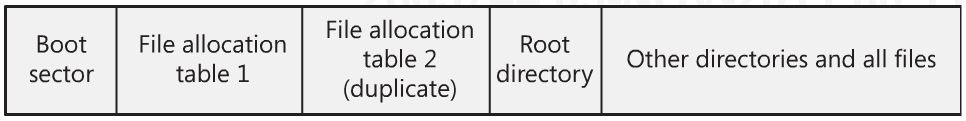
\includegraphics[width=12cm]{images/filesystem/fat_structure.jpg}
    \setcaptioncitation{https://social.technet.microsoft.com/wiki/contents/articles/6771.the-fat-file-system.aspx}
    \caption{Structure of a fat disk}
    \label{fig:galaxy}
\end{figure}


The FAT file system uses a file allocation table to keep track of the location of files and directories on the storage media. This table is essentially a map that lists the clusters (blocks of storage space) that are allocated to each file and directory on the disk.
One of the key features of the FAT file system is its use of \texttt{8.3 filenames}, which are filenames consisting of up to eight characters followed by a three-character extension. This limit on the length of filenames and the use of a limited character set (only uppercase letters, numbers, and a few special characters) was a limitation of early computing hardware but has since become a standard that is still used today. One of the extra milestones was to implement long entries in the filename to overcome this limitation.

\begin{figure}[htp]
    \centering
    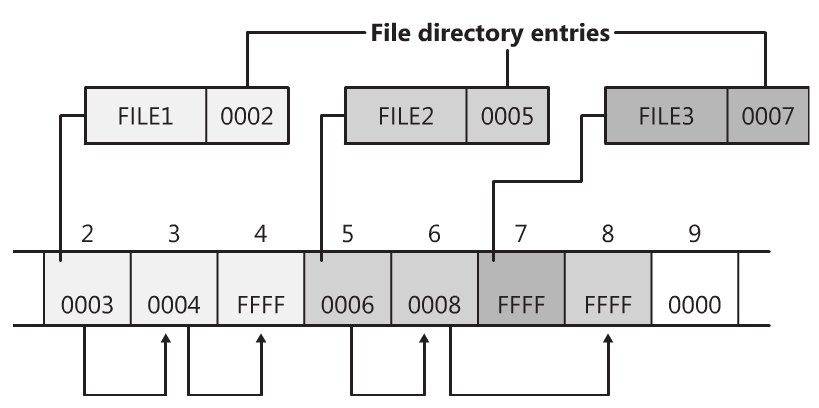
\includegraphics[width=12cm]{images/filesystem/fat_example.png}
    \setcaptioncitation{https://social.technet.microsoft.com/wiki/contents/articles/6771.the-fat-file-system.aspx}
    \caption{Example of a fat table}
    \label{fig:galaxy}
\end{figure}


The \href{https://fr.wikipedia.org/wiki/FAT32}{\texttt{FAT32}} file system is an updated version of the original FAT file system and includes several key differences compared to other FAT filesystems, such as \href{https://fr.wikipedia.org/wiki/FAT12}{\texttt{FAT12}} and \href{https://fr.wikipedia.org/wiki/FAT16}{\texttt{FAT16}}
\begin{itemize}
    \item Maximum partition size: One of the key differences between FAT32 and earlier FAT filesystems is the maximum \texttt{partition size}. FAT12 and FAT16 have limitations on the size of the partition they can support. FAT12 supports partitions up to 16MB, while FAT16 supports up to 2GB. FAT32, on the other hand, supports partitions up to 2 terabytes (TB). 
    \item Cluster size: Another difference between FAT32 and earlier FAT filesystems is the  \texttt{cluster size}. In FAT12 and FAT16, the cluster size is fixed, meaning that the entire partition is divided into clusters of a specific size. However, in FAT32, the cluster size can be adjusted to match the size of the partition. This can help improve the efficiency of the file system by reducing the amount of wasted space on the disk. In the SD card used for the tests, the cluster size was 4096 bytes divided into 8 sectors of 512 bytes.
    \item File and directory size limits: FAT12 and FAT16 have limitations on the maximum size of individual files and directories. FAT12 supports file sizes up to 32MB, while FAT16 supports file sizes up to 2GB. In addition, both FAT12 and FAT16 have limitations on the number of files and directories that can be stored on a partition. FAT32 removes these limitations, allowing for larger files and more files and directories on a single partition.
\end{itemize}
    
In summary, FAT32 offers several key improvements over earlier FAT filesystems, including support for \texttt{larger partitions}, \texttt{larger files and directories}, and \texttt{improved performance}.

\subsection{Understanding the fat32 specification}

Understanding the fat32 specification was a daunting task. I divided this big task into multiple parts:

\begin{itemize}
    \item  Gather some resources about fat32 on the internet. I found multiple websites that helped me to better understand the fat32 specification. 
    \item  Then I tried to get the big picture. How does fat32 work? What are key concepts?
    \item  Looked up unfamiliar terms. What is a cluster? What is a sector? A lot of terms were unknown to me at the beginning, and I had to learn all of them.
    \item Then I broke down each section into smaller, more manageable sections. It helped me to understand fat32 step by step.
    \item I began tackling the helper functions, which proved to be simpler and facilitated a seamless transition into the realm of fat.
    \item In the end, I completed the implementation of the FAT32 functions, starting with the reading functions and concluding with the writing functions.
\end{itemize}

\subsection{The actual implementation}

The implementation of the \texttt{fat32.c} file spans an extensive codebase comprising more than 2000 lines, making it impractical to provide a comprehensive explanation within the confines of this report. However, this section aims to shed light on the key aspects and main lines of the implementation. For a more thorough understanding, interested readers are encouraged to delve into the intricacies by browsing the source code directly.

Despite the complexity of the implementation, it is possible to discern an overarching structure that can be roughly categorized into three distinct sections. These sections delineate fundamental components and crucial operations that collectively form the larger picture of the \texttt{fat32.c} implementation.

While this report may not delve into the intricate details of each line of code, it seeks to provide a high-level overview and highlight the main elements and concepts of the implementation. By exploring these key components, readers can gain a solid grasp of the underlying principles and functionalities driving the \texttt{fat32.c} file.

\subsection{The data structures used in the filesystem}

\subsubsection{fat32\_filesystem}

The fat32 implementation has three distinct data structures that play a crutial role. The first among them is the \texttt{fat32\_filesystem} structure. This particular structure encapsulates crucial details and metadata that are fundamental to the functioning and management of the fat system as a whole. Without this data structure, we wouldn't be able to convert the lba address of a cluster number. By encompassing critical information, the \texttt{fat32\_filesystem} structure forms a foundational component, facilitating the overall organization, operation, and accessibility of data within the fat32 implementation.

\begin{lstlisting}[caption={fat32\_filesystem},captionpos=b,language=C,frame=single,breaklines]
struct fat32_filesystem {
    struct block_driver *b_driver;
    struct fat32_entry root_directory;
    uint32_t cluster_begin_data;
    uint32_t sectors_per_fat;
    uint32_t first_cluster_root_directory;
    uint8_t  sectors_per_cluster;
    uint16_t numbers_sectors_reserved;
    uint8_t  fat32_number;
    uint32_t next_free_cluster_hint;
};
\end{lstlisting}

\subsubsection{fat32\_entry}

The \texttt{fat32\_entry} data structure is specifically designed to work with fat32. It is connected to fat32 in a way that prevents the compiler from optimizing it (using the packed keyword), ensuring its essential role. The purpose of \texttt{fat32\_entry} is to uniquely identify a specific entry, such as a file or folder, within the fat32 system. We can draw an analogy to the primary key in a database.. When a program possesses a value of \texttt{fat32\_entry}, it becomes capable of accessing and reading the corresponding file or folder, regardless of the specific implementation being used. This connection between \texttt{fat32\_entry} and the associated entities enables seamless retrieval and interpretation of data within the fat32 system.

\begin{lstlisting}[caption={fat32\_entry},captionpos=b,language=C,frame=single,breaklines]
struct fat32_entry {
    char name[11];
    uint8_t attribute;
    uint8_t reserved_zero_entry;
    uint8_t creation_time;
    uint8_t empty[6];
    uint16_t cluster_high;
    uint16_t last_modifier_time;
    uint16_t last_modified_date;
    uint16_t cluster_low;
    uint32_t file_size;
} __attribute__((packed));
\end{lstlisting}

\subsubsection{fat32\_handle}

In simple terms, the \texttt{fat32\_handle} is a structure that helps us identify a specific entry, such as a file or directory, and enables us to interact with it. The key distinction between fat32\_entry and \texttt{fat32\_handle} is that the former is in a sense "stateless", meaning it only provides identification information, while the latter stores additional state information alongside it. This stored state allows us to have certain effects or keep track of specific information related to the entry.

For instance, with \texttt{fat32\_handle}, we can maintain the position of a cursor within a file, which is useful for seeking to different parts of the file. It can also help us keep track of the current directory by storing an index, which is beneficial for reading directory contents.

The primary purpose of the \texttt{fat32\_handle} structure is to facilitate communication and interaction with the library built on top of it. By utilizing \texttt{fat32\_handle}, we can effectively perform various operations and access specific functionalities provided by the library. It serves as a helpful tool for managing the state and accessing relevant information associated with a particular entry in the fat32 file system.

\begin{lstlisting}[caption={fat32\_handle},captionpos=b,language=C,frame=single,breaklines]
struct fat32_handle {
    // Current entry
    struct fat32_entry entry;
    // Information about the cluster
    uint32_t current_cluster;
    uint32_t relative_sector_from_cluster;
    // Information for the c library on top of it
    union {
        uint32_t directory_offset;
        uint32_t file_position;
    };
    char *path;
    bool is_directory;
    // Entries about the parent - required to modify entry
    uint32_t parent_cluster_number;
    uint32_t parent_cluster_offset;
};
\end{lstlisting}

\subsection{Functions used to implement the filesystem}

The functions in the implementation can be broadly classified into three main categories.

The first category consists of \textbf{helper functions}. These functions are designed to assist in carrying out more complex routines. They do not produce any side effects or make any modifications to the system. Instead, they provide support and aid in performing specific tasks within the implementation.

The second category comprises functions that are responsible for \textbf{performing operations on the fat32 file system}. These functions directly interact with the file system, executing actions such as reading, writing, or modifying data within the fat32 structure. They play a crucial role in ensuring the proper functioning and manipulation of the file system.

The third and final category encompasses functions that fulfill the specific requirements of the library, allowing it to effectively \textbf{interact with the file system}. These functions are tailored to meet the needs and demands of the library, providing the necessary functionalities and interfaces for seamless communication between the library and the underlying file system.

\subsubsection{Helper functions}

The first part consists of helper functions. These functions don't cause any problems and are used for three important reasons:
\begin{itemize}
    \item Improved readability: When we read the source code of a function, having helper functions makes it easier to understand what the function does. It helps us quickly grasp the purpose and functionality of the code. 

    \item Avoiding duplication: By using helper functions in multiple places, we can avoid repeating the same code over and over again. This saves us time and effort, making the code more efficient and manageable.

    \item Easier testing and bug detection: Helper functions can be tested more easily and independently. This allows us to identify and fix any errors or bugs in the code more quickly. By isolating specific functionalities in helper functions, we can focus on testing them individually and ensure their reliability. It enables us to employ unit tests as well.

    \item Overall, employing helper functions simplifies the code, promotes code reuse, and enhances the efficiency of testing and bug detection processes.
\end{itemize}

\begin{lstlisting}[caption={Example of unit test (true or false indicates if the name is for a directory)},captionpos=b,language=C,frame=single,breaklines]
void _test_name_valid(void) {
    // Test filenames - examples from here (http://elm-chan.org/docs/fat_e.html)
    assert(is_fat32_name_valid("FILENAME.TXT", false));
    assert(!is_fat32_name_valid("FILENAME.TXT", true));
    assert(is_fat32_name_valid("file.txt", false));
    assert(!is_fat32_name_valid("file.txt", true));
    assert(is_fat32_name_valid("NOEXT", true));
    assert(!is_fat32_name_valid(".cnf", true));
    assert(!is_fat32_name_valid(".cnf", false));
    assert(!is_fat32_name_valid("new file.txt", false));
    assert(!is_fat32_name_valid("new file.txt", true));
    assert(!is_fat32_name_valid("file[1].2+2", false));
    assert(!is_fat32_name_valid("two.dots.txt", false));
    assert(!is_fat32_name_valid("two.dots", true));
    return;
}
\end{lstlisting}


\subsubsection{Functions that perform operations on the fat32 filesystem}

The second category of functions includes those that perform specific operations within the fat32 system, but are not directly related to user actions like opening files, reading, or creating directories. These functions handle internal tasks that are essential for the proper functioning of the fat32 system.

For example, one function in this category is \texttt{get\_next\_cluster}. This function is responsible for reading the content of the next cluster when provided with a cluster number. Another function, \texttt{fat32\_remove\_chain}, is another example. It is designed to delete an entire chain of clusters and update the system's state by writing changes to the disk.

Among all the functions in this category, two hold particular significance. They are used in multiple other functions and play a critical role in the fat32 system. These functions require special attention and scrutiny because if they contain any bugs or errors, the entire file system may quickly become unstable. This could result in the violation of important invariants required by the fat32 system, rendering it in an undefined or an inconsistent state.

\subsubsection{fat32\_resolve}

When we talk about resolving a path in the fat32 filesystem, it means finding the exact location or full path of a file or directory based on the given path. A path is like a set of directions that tells us where a file or directory is in relation to the main or root directory of the filesystem.

The function \texttt{fat32\_resolve} is responsible for this task. It takes a path as input and returns a handle, which is like a reference or pointer, to the file or directory that matches the given path. However, if the input path is not valid or doesn't exist, \texttt{fat32\_resolve} will give an error instead of a handle.

To understand how \texttt{fat32\_resolve} works, we can look at its pseudo code. This pseudo code is a simplified version of the actual code that explains the steps and logic used in the function to resolve the path and find the corresponding file or directory.

\begin{algorithm}
\caption{Resolve path}
\begin{algorithmic}
\Procedure{fat32\_resolve\_path}{$\text{path}, \text{handle}$}
    \State \Call{assert}{path\_is\_absolute}
    
    \While{not \Call{is\_path\_end}{}()}
            \State $\text{current\_path}, \text{next\_path} \gets \text{split\_path}()$
            
            \State $\text{not\_found} \gets \Call{find\_directory}{\text{current\_path}}$
            \If{$\text{not\_found}$}
                \Return $\text{FS\_ERR\_NOTFOUND}$
            \EndIf
            \If{\Call{is\_file}{$\text{current\_path}$} \textbf{and} \Call{is\_not\_last}{}()}
                \State \Return $\text{FS\_ERR\_NOTDIR}$
            \EndIf
            
            \State $\text{path} \gets \text{next\_path}$
    \EndWhile

    \State \Call{fill\_handle}{handle}
\EndProcedure
\end{algorithmic}
\end{algorithm}

\subsubsection{fat32\_find\_directory}

The second essential function is designed to \texttt{traverse} through a directory's files and perform a specific function or operation on it. It essentially goes through each entry, one by one, and executes the provided function for each entry. This function operates as a loop, ensuring that the desired operation is carried out on all the folders within the directory.

To understand the inner workings of this function, we can refer to its pseudo code. This code provides a simplified explanation of the steps and logic involved in executing the function and performing the desired operation.

In summary, the first function helps us navigate paths, while the second function allows us to \texttt{iterate} through a directory's entries and perform a specified operation on each entry.

\begin{algorithm}
\caption{fat32\_find\_directory}
\begin{algorithmic}[1]
\Procedure{fat32\_find\_directory}{path, directory\_entry}
    \State $next \gets \text{true}$
    \State $current\_cluster\_number \gets \text{get\_cluster\_number}()$
    \State $lba\_start \gets \text{get\_lba\_from\_cluster}(current\_cluster\_number)$

    \While{$next$}
        \For{$j \gets 0$ to $sectors\_per\_cluster$}
            \State $\text{read\_block}(lba, data)$

            \For{$i \gets 0$ to $number\_directories\_per\_block$}
                \State $current\_entry \gets data[i]$

                \If{$\text{compare\_filename\_with\_entry}(current\_entry, path)$}
                    \State $directory\_entry \gets current\_entry$
                    \State \textbf{return}
                \EndIf

                \If{$current\_entry.\text{name}[0] == END\_DIRECTORY$}
                    \State \textbf{return} $FS\_ERR\_NOTFOUND$
                \EndIf
            \EndFor
        \EndFor

        \If{$lba\_start == cluster\_begin\_data$}
            \State $next \gets 0$
            \State \textbf{continue}
        \EndIf

        \State $\text{fat32\_get\_next\_cluster}(current\_cluster\_number, next\_cluster\_number)$

        \If{$next\_cluster\_number \geq END\_CLUSTER$}
            \State $next \gets 0$
        \EndIf
    \EndWhile
\EndProcedure
\end{algorithmic}
\end{algorithm}

 \subsubsection{Final words}

As a programmer, I want to emphasize that all functions are important, and I haven't overlooked the significance of the other functions. However, let's add a touch of humor to this section of the report. Imagine if the incredible team at AOS gives a magical oracle that could instantly generate a ready-to-use code with exactly two perfectly correct functions. We are allowed to get two functions. In that imaginary scenario, these two functions would undeniably be the two I would ask by writing to the staff.

\subsubsection{The last category}

The final group of functions includes those that perform specific operations on the fat32 and will act similar to an \texttt{entry point}. These functions are designed to carry out various \texttt{tasks} within the fat32 system.

The table below provides an explanation of what each function does, outlining their respective functionalities. These functions are accessed through RPC using the \texttt{aos\_rpc} framework and the library implemented in fopen.

In simpler terms, these functions are like tools that can be used as \texttt{entry point} by other processes to interact with and perform operations on the fat32 system. They offer a range of functionalities that can be accessed remotely through a library, making it easier for different processes to manipulate the fat32 system.

\begin{lstlisting}[caption={"Entry points" in the filesystem},captionpos=b,language=C,frame=single,breaklines]
errval_t fat32_open(struct fat32_filesystem *fs, const char *path, struct fat32_handle **handle);
errval_t fat32_close(struct fat32_filesystem *fs, struct fat32_handle *handle);
errval_t fat32_stat(struct fat32_filesystem *fs, const struct fat32_handle *handle, struct fs_fileinfo *info);
errval_t fat32_read(struct fat32_filesystem *fs, struct fat32_handle *handle, void *data, size_t size, size_t *nb_bytes_read);
errval_t fat32_write(struct fat32_filesystem *fs, struct fat32_handle *handle, const void *data, size_t size, size_t *nb_bytes_written);
errval_t fat32_seek(struct fat32_filesystem *fs, struct fat32_handle *handle,enum fs_seekpos whence,off_t offset);
errval_t fat32_tell(struct fat32_filesystem *fs, struct fat32_handle *handle, size_t *pos);
errval_t fat32_open_directory(struct fat32_filesystem *fs, const char *path, struct fat32_handle **handle);
errval_t fat32_close_directory(struct fat32_filesystem *fs, struct fat32_handle *handle);
errval_t fat32_read_next_directory(struct fat32_filesystem *fs, struct fat32_handle *handle, char **new_name);

errval_t fat32_remove(struct fat32_filesystem *fs, const char *path);
errval_t fat32_remove_directory(struct fat32_filesystem *fs, const char *path);
errval_t fat32_create(struct fat32_filesystem *fs, const char *path, struct fat32_handle **handle);
errval_t fat32_mkdir(struct fat32_filesystem *fs, const char *path, struct fat32_handle **handle);
\end{lstlisting}

\subsubsection{Concurency inside the filesystem}

In a real-world operating system, multiple users can \texttt{simultaneously} write to a file. This necessitates the capability to handle \textbf{concurrent requests} to the file system without compromising its integrity. To address this, the implemented solution utilizes a large lock encompassing the entire file system. When a function is invoked from the \texttt{aos\_rpc} framework, it is locked by this mechanism. Alternatively, a read-write lock can be employed, as interleaved multiple reads pose no problems. However, the main concern lies with the write operations, for which locking is crucial. This approach mirrors the principles employed in other concurrent algorithms. 

\subsubsection{Do we really need lock in our case? - analogy with golang channels}

\href{https://go.dev/}{Go (Golang)}   is a programming language developed by Google. It focuses on simplicity, efficiency, and concurrency. It features a garbage collector, built-in concurrency primitives, and is widely used for web development, systems programming, and networking applications.

In \href{https://go.dev/}{\texttt{Go (Golang)}, \href{https://www.educative.io/answers/what-is-a-goroutine}{\texttt{a goroutine}} is a lightweight concurrent execution unit. It is a function or method that can be launched independently and run concurrently with other goroutines within the same program. Goroutines are managed by the Go runtime and utilize a small amount of memory, allowing for the creation of thousands or even millions of goroutines. They are designed to efficiently handle concurrent tasks, enabling concurrent programming without the overhead of traditional threads. Goroutines communicate with each other using channels, which provide synchronized and safe communication between concurrent goroutines. The combination of goroutines and channels forms the foundation of Go's powerful concurrency model.

In Go (Golang), \href{https://www.educative.io/answers/what-are-channels-in-golang }{\texttt{channels}} are a fundamental feature used for communication and \texttt{synchronization} between goroutines. A channel is a typed conduit that allows for the sending and receiving of values between concurrent goroutines. It provides a safe and efficient way to exchange data and coordinate actions among goroutines.

In Golang, there are essentially two main techniques to lock a critical section within a code snippet. The first approach involves using a traditional mutex, similar to other programming languages. However, Golang offers a remarkably elegant solution (in my honest opinion) using channels. In this method, all goroutines (referred to as threads in Golang jargon) send their requests through a channel. Subsequently, another goroutine situated at the channel's endpoint processes the received requests sequentially, ensuring that the actions are executed \textbf{in a sequential order and avoiding any interleaving of two critical sections}.

Now comes a fundamental question: Is it really necessary to have a \textt{lock} in our function? Upon closer examination, I fail to identify any scenario where two requests to the initialization process could execute code in an interleaved manner. Why is this the case? Well, all calls to the filesystem within the function are \textbf{blocking} and operate on a \textbf{completion basis}. This means that we only exit the \texttt{critical section} in two situations: when the call is completed successfully or when an error occurs. In both cases, the execution of the function concludes, allowing the next request to enter the \texttt{critical section}. Consequently, we encounter \textbf{no interleaving}. It is important to note that the filesystem and block driver are exclusively present in the init process. While discussing Golang within this report may seem surprising, upon reflection, we can indeed see that the concurrency pattern we are encountering aligns precisely with goroutines and channels in Golang.

Let's approach this question from a critical standpoint. Does having a lock-free filesystem imply that I am the next superstar PhD student in systems? Absolutely not. If the current operating system we have developed were to adopt such an \texttt{architecture}, we would consider the design to be mediocre (in a real world setup). The only reason I can consider avoiding locks in this particular case is due to two specific properties. Firstly, the filesystem (which is the sole component we need to trust in order to maintain FAT32 invariants) resides in the init process. Secondly, all calls to this component are blocking and execute upon completion. It is these two properties that enable me to eliminate the need for locks in this context. In scenarios where the block driver is in a waiting state, incorporating a non-blocking call would enable another process to execute computations during the waiting period. However, adopting this approach would necessitate the implementation of a file system lock to ensure proper synchronization and prevent data integrity issues. 
\subsection{Communication with the read world}

We now have a fully functional file system that allows us to perform various operations like reading, writing, adding and deleting directories. However, it would be unwise to assume that our work is complete.

Initially, our file system is only accessible to the init process and is not visible to the rest of the operating system. To make the most of its functionality, we need to establish a gateway for our file system. The question arises: How should we integrate the file system? Should it be as a library that other processes can utilize? Should we use RPC calls and centralize everything within the init process?

\subsubsection{A full barrelfish library}

The first idea is quite creative. It suggests having a basic service, called the block driver, residing in the init process. Any application that wants to work with the fat32 formatted disk could include a specific file, like "fat32.h," and directly call functions to manipulate the disk using a pointer to the block driver. To ensure safe communication between multiple processes, the critical part of the block driver would be protected by a lock.

Although this idea remains at the conceptual stage and may seem eccentric and challenging to implement, it serves the purpose of exploring different operations and ideas. Without the exposure to Barrelfish and this course, I would have likely stuck to more conventional Unix-based approaches and not considered such unconventional ideas.

Taking time to ponder this idea, I see potential benefits. In an operating system like \href{https://barrelfish.org/}{\texttt{Barrelfish}}, which is a \href{https://en.wikipedia.org/wiki/Microkernel}{\texttt{microkernel}} offering flexibility and unique behaviors compared to \href{https://en.wikipedia.org/wiki/Monolithic_kernel}{\texttt{monolithic kernels}} like Linux, there are advantages to be found. For instance, imagine an application with heavy input/output (I/O) demands. By directly interacting with the block driver, each call can \texttt{bypass} the \texttt{overhead} of RPC calls, saving valuable time and system resources. Another advantage is that the file system is implemented as a \texttt{library}. Skilled programmers could \texttt{customize} and optimize this library for specific application patterns, enhancing performance for specific tasks.

In conclusion, this eccentric idea showcases how a system like \texttt{Barrelfish} fosters the imagination of diverse computer systems. By moving a significant portion of the kernel into \texttt{userspace}, it provides additional flexibility and opens up possibilities for innovative approaches.


\subsubsection{A single service that lies in the init process}

The second idea and solution involve integrating the filesystem directly into the init process alongside the block driver. Any process that wants to interact with the filesystem will simply use a \texttt{high-level API} to make RPC calls for their requests. This design decision is less unique compared to the first idea and resembles the structure found in \href{https://fr.wikipedia.org/wiki/Unix}{\texttt{UNIX-like systems}}.

There are a few reasons why I chose this approach. Firstly, it aligns with the overall consistency of our system, which is important for simplifying our RPC infrastructure. Since all services are contained within the init process, this design decision maintains consistency within our team. However, it does have its drawbacks and disadvantages, and whether it is the right choice remains uncertain. Nonetheless, since we decided on this direction, it makes sense for me to follow the same approach for my individual milestone.

Another factor to consider is the available time. Building and integrating a fat32 file system is a complex software engineering project, not just a simple coding exercise. Like any other project, time constraints must be taken into account. Choosing a more standard design provides assurance that the project will yield results and have fewer surprises compared to a more creative implementation.

Therefore, I implemented all the necessary parts in the \texttt{fat32.c} file to enable interaction with the block driver and perform operations within the filesystem. The filesystem includes a pointer to an instance of the block driver, which allows it to read and write blocks on the disk.

\subsubsection{The "C" Api}

The "C" API in \texttt{fopen.c} is a collection of functions and data structures that allow the shell and other processes to interact with the fat32 file system in a \texttt{standardized} way. It provides a clear and defined interface for communication. This standardized interface ensures that multiple processes can access files and directories simultaneously, enabling them to read from and write to the file system.

The filesystem API includes various functions for different operations. For example, there are functions for creating, opening, reading, writing, and closing files. Additionally, there are functions specifically designed for working with directories, such as creating new directories, listing directory contents, and retrieving file attributes.

By using the filesystem API in userspace, processes can perform a wide range of tasks related to working with files and directories. This includes tasks like copying files, creating new directories, and viewing the contents of a directory. The API provides a consistent and reliable way for processes to interact with the fat32 file system, making it easier to manage and manipulate files and directories in a standardized manner.

The "C" API serves as a wrapper that adds additional functionality and acts as a bridge between a \texttt{Barrelfish} process and the \texttt{aos\_rpc} framework. This API facilitates the communication between the process and the filesystem by sending RPC calls through our \texttt{aos\_rpc} framework.

\begin{lstlisting}[caption={Function filled in libopen},captionpos=b,language=C,frame=single,breaklines]
static int fs_libc_open(char *path, int flags);
static int fs_libc_read(int fd, void *buf, size_t len);
static int fs_libc_write(int fd, void *buf, size_t len);
static int fs_libc_close(int fd);
static off_t fs_libc_lseek(int fd, off_t offset, int whence);

static errval_t fs_mkdir(const char *path);
static errval_t fs_rmdir(const char *path);
static errval_t fs_rm(const char *path);
static errval_t fs_opendir(const char *path, fs_dirhandle_t *h);
static errval_t fs_readdir(fs_dirhandle_t h, char **name);
static errval_t fs_closedir(fs_dirhandle_t h);
static errval_t fs_fstat(fs_dirhandle_t h, struct fs_fileinfo *b);
\end{lstlisting}

\subsubsection{Benchmarking the filesystem}

Benchmarking the filesystem lacks a singular definitive approach due to the presence of numerous viable methods to evaluate its performance. Consequently, during the benchmarking process, three distinct decisions were made to ensure a clear and rigorous evaluation of the filesystem's performance.

The initial decision made during the benchmarking process involves opting not to test the filesystem exclusively from the fopen functions but instead directly evaluating the \texttt{fat32.c} file itself. This choice is driven by the consideration of \texttt{dependencies} and their potential impact on the observed performance. To illustrate this, let's consider two scenarios.

In the first scenario, let's assume we have an exceptionally fast implementation of an RPC call. If we were to benchmark the filesystem solely based on the \texttt{fopen.c} functions, the overall filesystem performance would appear faster due to the swift execution of the RPC call. However, this may not accurately reflect the \texttt{true performance} of the filesystem as a whole.

It is essential to recognize that the RPC handler is an \texttt{external component} that is \texttt{extrinsic} to the filesystem. Thus, any fluctuations in its speed can distort the perception of the filesystem's performance. By testing directly from the \texttt{fat32.c} file and bypassing the specific dependency of the RPC handler, we aim to obtain a more \texttt{accurate} evaluation of the filesystem's performance, unadulterated by the potential confounding effects of external components.

The second decision made in the benchmarking process pertains to the evaluation of \texttt{peak performance} concerning the actual number of \texttt{bytes read} and \texttt{written} to the disk \texttt{per second}. This particular assessment falls under the purview of benchmarking the block driver, not the filesystem itself. It is important to note that the end user's primary concern does not lie in the speed of writing data in terms of bytes per second. In fact, what truly matters in the testing of the filesystem is the speed in cycles required to read from and write to a file.

To illustrate this concept, let's consider a scenario where we have an exceptionally fast block driver, assuming it is ten times faster for the sake of simplicity. Additionally, let's assume that the underlying fat implementation, on average, needs to read ten blocks to access a file of size X. Now, contrast this with a normal block driver that is ten times slower than the aforementioned faster version. In this case, however, the fat implementation only needs to read one block, on average, to access the same file of size X.

In the first scenario with the faster block driver, the overall bandwidth appears more aggressive due to its heightened performance capabilities. However, from the user's perspective, there is no noticeable difference in speed. The perceived speed experienced by the user remains the same in both situations, regardless of the variation in the underlying block driver's performance.

The last decision worth mentioning is that we conduct filesystem testing when there are only a few entries on the disk. This is important because when we write to a new file, it may take longer if we need to locate a new cluster, for instance. In the worst-case scenario, we would have to iterate through the entire FAT32 table entry, which can be a time-consuming process. On the other hand, in a more optimistic scenario, we can find a free entry within the same block if we need to extend the file's size, resulting in a faster operation. It's worth noting that these measurements were performed on a \texttt{freshly formatted filesystem}.

To conclude, \textbf{benchmarking the block driver} primarily revolves around evaluating the \textbf{"true" speed}, which encompasses the actual number of bytes written to the disk per second. On the other hand, \textbf{benchmarking the filesystem} focuses on assessing the \textbf{perceived speed minus the RPC overhead} experienced by the user, which considers the speed in cycles required for reading from and writing to files. We get a max read bandwith around \texttt{1350 bytes per second} without caching and around \texttt{100 gigabytes per second} with caching and perfect temporal locality. The writes are a bit slower. We manage to reach \texttt{900 bytes per second without caching} and \texttt{1350 bytes per second with caching}.



\begin{figure}[htp]
    \centering
    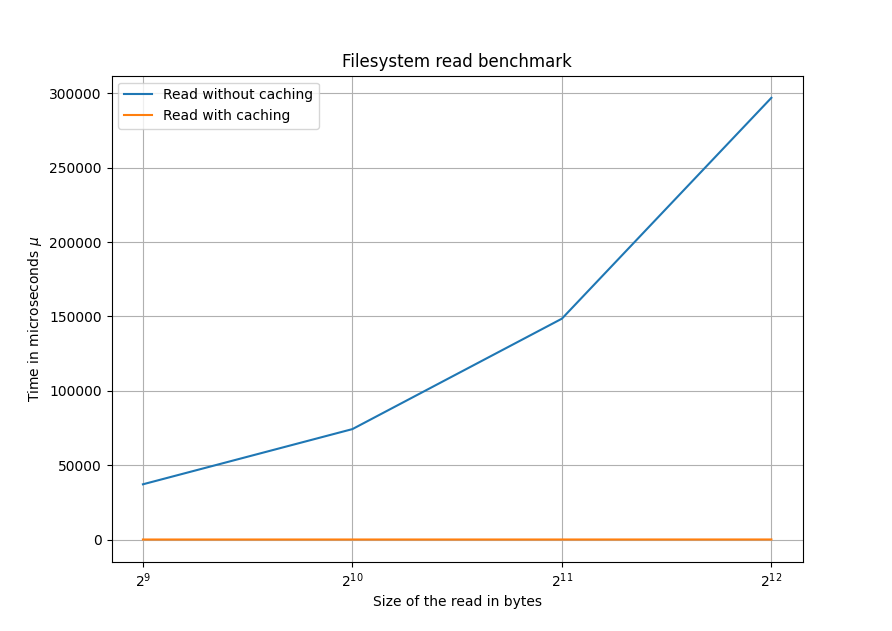
\includegraphics[width=12cm]{images/filesystem/filesystem_benchmark_read.png}
    \caption{Benchmark filesystem read}
    \label{fig:galaxy}
\end{figure}


\begin{figure}[htp]
    \centering
    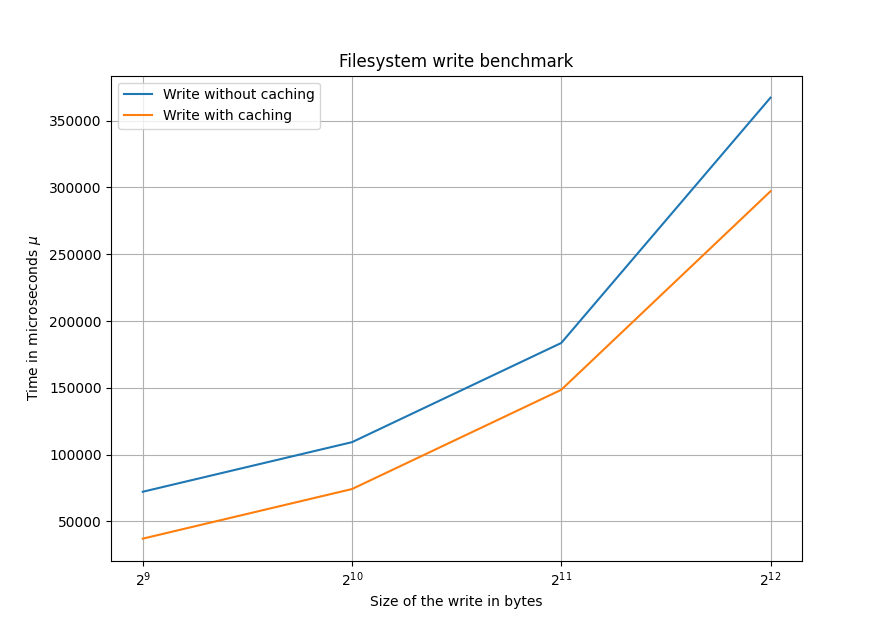
\includegraphics[width=12cm]{images/filesystem/filesystem_benchmark_write.png}
    \caption{Benchmark filesystem write}
    \label{fig:galaxy}
\end{figure}

We can also import elf entries from the computer's file system. ELF files are binary files similar to others, so it makes sense that we can import them from the file system. However, because our block driver is not very fast, importing an elf binary takes some time. It usually takes about one minute for a simple program to import. Here's how the importing process works:

In the process manager, we first check if the name of the binary starts with "/sdcard/". If it does, we import it from the file system using that specific location. Otherwise, we import it from the multiboot options as usual. The process loader module \textfff{dynamically} handles requests to load binary data.

\begin{lstlisting}[caption={Routing the load request to the correct source},captionpos=b,language=C,frame=single,breaklines]
static errval_t _load_elf_internal(const char *path, struct elfimg *img, int *argc, char ***argv) {
    if((strnlen(path, 7) >= 7 && strncasecmp("/SDCARD/", path,7) == 0)) {
        return spawn_load_filesystem(path, img, argc, argv);
    } else {
        return spawn_load_elf(bi, path, img, argc, argv);
    }
}
\end{lstlisting}

\subsubsection{Last but not least, the integration with the shell}

Upon completion of the block driver, a crucial component of our operating system is now \texttt{operational}. However, it is important to note that this achievement does not mark the end of our journey. There remains an open question regarding how we seamlessly \texttt{integrate} this component into \texttt{the broader system}, particularly in terms of \texttt{communication} with the shell.

The integration of the filesystem itself did not pose a significant challenge. Fortunately, the file \texttt{fopen.c} served as a suitable interface, bridging the gap between the shell and the filesystem. By combining these two entities, we were able to establish a connection that allowed for the smooth functioning of the filesystem. Although minor issues surfaced during this integration process, overall, the filesystem performed admirably.

The integration of the filesystem within the shell environment provided us with an opportunity to thoroughly test and expand upon some of the shell's built-in functionalities, such as \texttt{ls} or \texttt{cat} This collaborative environment enabled us to uncover additional issues within the filesystem and address them accordingly. It served as a fertile ground for identifying any potential shortcomings and further refining the filesystem's overall functionality.

\begin{figure}[htp]
    \centering
    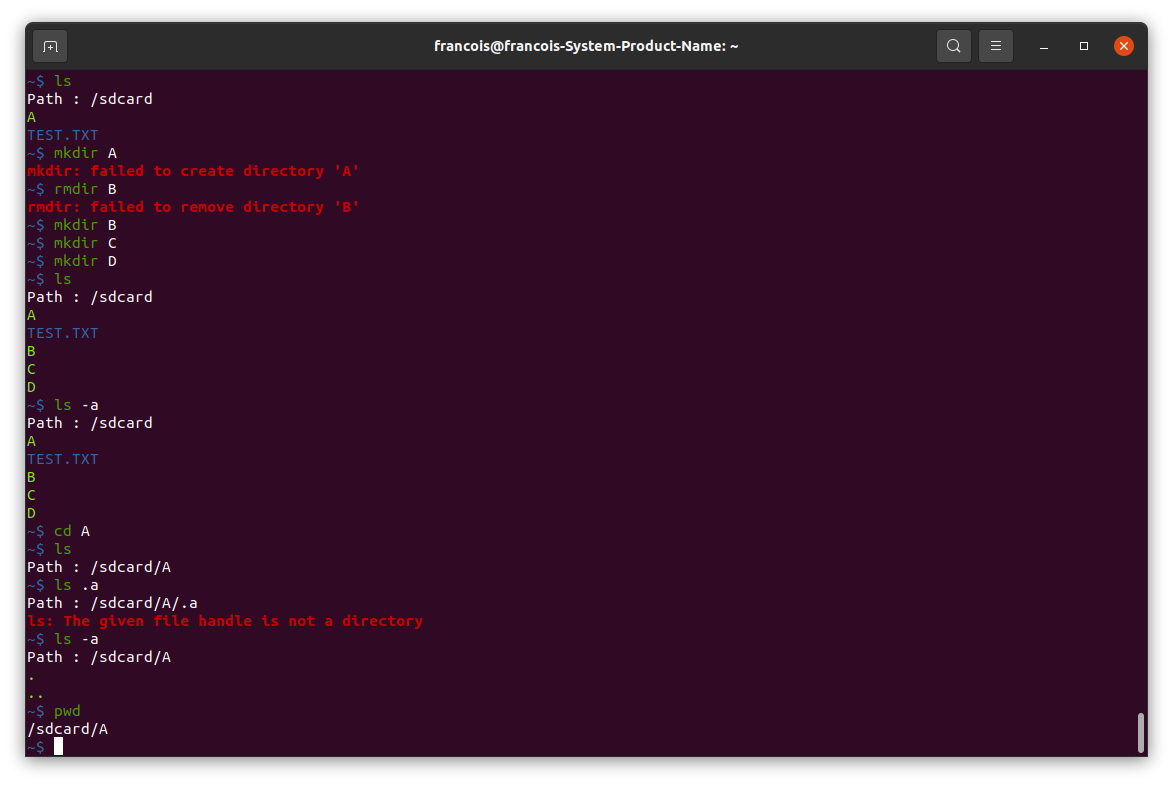
\includegraphics[width=12cm]{images/filesystem/interaction_with_shell.png}
    \caption{Interaction with the shell}
    \label{fig:galaxy}
\end{figure}


\begin{figure}[htp]
    \centering
    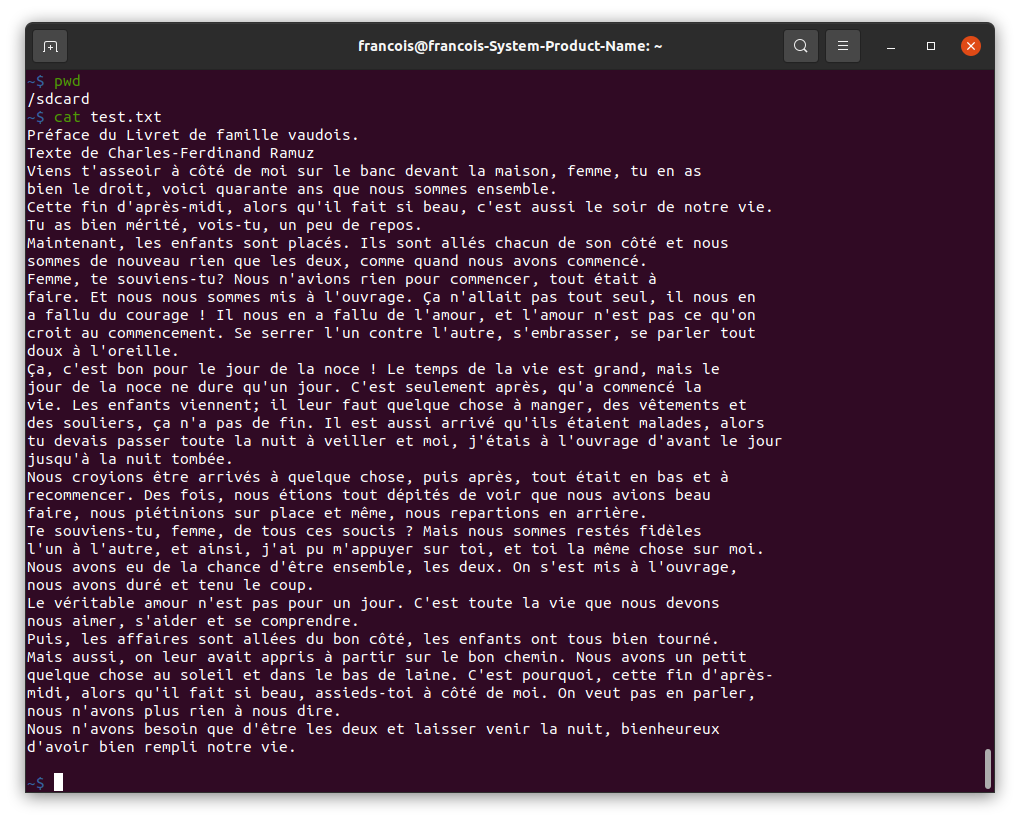
\includegraphics[width=12cm]{images/filesystem/example_cat.png}
    \caption{Cat}
    \label{fig:galaxy}
\end{figure}


\section{Conclusion and next steps}

\subsection{Limitations of our filesystem}

Presently, our filesystem exhibits certain limitations. Listed below are the limitations that we should consider.

\begin{itemize}
    \item The maximum allowed character limit for paths, including the mounting point, is 512 characters.

    \item Our current system lacks support for long filename entries, and we are constrained to adhere to the 8.3 FAT naming convention.

    \item When a directory containing files is deleted, it results in a leak in the FAT table. To mitigate this issue, we can enforce a restriction where users are only allowed to remove empty directories.

    \item Our system currently does not provide support for any timestamps.
\end{itemize}


\subsection{Possible improvements}

Creating a fat32 filesystem was a \texttt{challenging task} that took me longer than expected. I had to write, rewrite, and test over \texttt{2800 lines of code} to reach an acceptable version.

Although the filesystem is functional, there are still areas that can be improved. Here are some potential next steps:

\begin{itemize}
    \item \textbf{Enhance the block driver}: The current block driver is not very fast, and there are several areas where it can be improved. For instance, we can optimize it by reading multiple sectors at once or increasing the device's speed.

    \item \textbf{Develop a more robust test framework}: It would be beneficial to have a simulated disk in the test framework. This way, we can perform operations on the simulated disk and verify if the required fat32 invariants are maintained.

    \item \textbf{Improve file metadata support}: Currently, some important file metadata information is missing. For example, we don't have information about when a file was created. Enhancing the filesystem to include better file metadata support would be beneficial.

    \item \textbf{Refine the code}: Given the time limitations, adhering to the best software engineering practices consistently proved challenging. Consequently, there is significant room for refactoring and improvement.

    \item \textbf{Support for long file name entries}: At present, our filesystem encounters two significant restrictions. Firstly, the path size must not exceed 512 characters. Additionally, we solely accommodate the 8.3 naming convention.
    
\end{itemize}


By addressing these areas of improvement, we can enhance the performance, reliability, and overall quality of the fat32 filesystem implementation.

\subsubsection{Enhance the block driver}

The block device driver we recieved is basic and slow but we can improve it. We can try different approaches to improve performance, such as reading or writing multiple blocks together, using interrupts instead of polling for data transfer, or adjusting the card's clock frequency through the host controller. 

There are still numerous opportunities for improvements within the block driver. One significant advancement would involve negotiating the optimal parameters with the hardware, aiming to achieve the most efficient and effective performance. Additionally, an enhancement worth considering is the implementation of a mechanism that allows for writing multiple blocks simultaneously. By leveraging this approach, we can further optimize data transfer and throughput, potentially enhancing the overall efficiency of the block driver.

\subsubsection{Develop a more robust test framework}

One potential approach we could take to enhance the testing of the \texttt{fat32\_filesystem} is by implementing a mock block driver. By doing so, we would create a simulated environment that emulates the behavior of the actual block driver. This would provide us with a valuable means of conducting unit testing for the \texttt{fat32\_filesystem}, allowing us to thoroughly evaluate its functionality and performance.

\subsubsection{Add metadata in the filesystem}

These entries are currently not included in my filesystem and implementation, but we could add them to the metadata of the files and directories in the FAT32 filesystem.

\begin{itemize}
    \item \textbf{Creation Date and Time}: This records the specific date and time when the file or directory was originally created.

    \item \textbf{Last Modified Date and Time}: This indicates the date and time when the file or directory was last modified or changed.

    \item \textbf{Access Date}: This denotes the date when the file or directory was last accessed or opened.
    
    \item \textbf{Permissions}: These define the access permissions for the file or directory, specifying who can read, write, or execute it.
\end{itemize}

\subsubsection{Improving the quality of the code}

Here are some ideas we can use to improve the quality of the code

\begin{itemize}
    \item \textbf{Modularize the code}: Break down the code into smaller, reusable modules or functions. This improves readability, maintainability, and allows for better code organization.

    \item \textbf{Use meaningful variable and function names}: Ensure that variable and function names accurately describe their purpose and functionality. This improves code comprehension and makes it easier to understand and work with the code.

    \item \textbf{Improve error handling}: Add more error-handling mechanisms throughout the code to handle exceptional scenarios gracefully. This includes handling file system errors, memory allocation failures, and input validation. Even if the code has some primitives for it, we could clearly extend it and make it better. We have no custom errors specific to our implementation.

    \item \textbf{Optimize performance}: Identify potential bottlenecks or areas where the code can be optimized for better performance. This could involve doing disk I/O operations, reducing unnecessary computations, and trying to find better data structures. Optimizing the search for a free cluster is a potential area for improvement.

    \item \textbf{Incorporate design patterns}: Study and apply relevant design patterns to enhance the overall architecture and structure of the filesystem code. Design patterns provide proven solutions to common software design problems and can improve code maintainability and extensibility.
\end{itemize}


\subsubsection{Support for long file name entries}

Currently, within our filesystem, we face two noteworthy limitations that impose certain constraints. Firstly, it is imperative to ensure that the size of the path does not surpass the threshold of \texttt{512 characters}. This restriction is in place to maintain the integrity and efficiency of file management operations within the system. Furthermore, it is important to note that our filesystem exclusively supports the utilization of the \texttt{8.3 naming convention}. This convention dictates that file and directory names consist of a maximum of eight alphanumeric characters, followed by a period, and a maximum of three alphanumeric characters as the file extension.

\section{Retrospective}

Creating the filesystem was a long task with lots of complexity. In total, I had to write 3000 lines of code in a short time. It was so important to get every single line right because even one bad line could break the fat32 invariants. Also some parts of the code could still be improved. For instance, when we make a new directory, we unnecessarily delete everything in the cluster. A lot of time were spent in carefully testing the filesystem to make sure it works well. In addition to that, it has been observed that the block driver is operating slowly, and there is potential for improvement by developing a more efficient driver.